\documentclass[a4paper, 12pt]{book}

\usepackage{fancyhdr}

\newcommand{\ttitle}{Bayesova statistika - zapiski s predavanj prof. Smrekarja}
\newcommand{\ttitleshort}{Bayesova statistika}
\newcommand{\tauthor}{Tomaž Poljanšek}
\newcommand{\tdate}{študijsko leto 2023/24}

\usepackage{color}
\usepackage{soul}
\usepackage[numbers]{natbib}

\usepackage{physics}

\usepackage[parfill]{parskip}
\usepackage[hyphens]{url}

\usepackage[usestackEOL]{stackengine}[2013-10-15] % formatting Pascal
\usepackage[dvipsnames]{xcolor}

\usepackage{cancel}
\usepackage[export]{adjustbox}

% Related to math
\usepackage{amsmath,amssymb,amsfonts,amsthm}
\usepackage{mathtools}
\usepackage{youngtab}
\usepackage{tikz}

% encoding and language
\usepackage{lmodern}
\usepackage[slovene, english]{babel}
\usepackage[utf8]{inputenc}
\usepackage[T1]{fontenc}

% multiline comments
\usepackage{comment}
\usepackage{verbatim}

% random text - for texting
\usepackage{lipsum}
\usepackage{blindtext}

\usepackage{hyperref}

% images
\usepackage{graphicx}
\graphicspath{ {../images/} }

% no blank page
\usepackage{atbegshi}
\renewcommand{\cleardoublepage}{\clearpage}

% theorems
\theoremstyle{definition}
\newtheorem{counter}{Counter}[section]
\newtheorem{defn}[counter]{Definicija}
\newtheorem{lemma}[counter]{Lema}
\newtheorem{conseq}[counter]{Posledica}
\newtheorem{claim}[counter]{Trditev}
\newtheorem{theorem}[counter]{Izrek}
\newtheorem{pro}[counter]{Dokaz}
%%
\theoremstyle{remark}
\newtheorem*{ex}{Primer}
\newtheorem*{exmp}{Zgled}
\newtheorem*{rem}{Opomba}

% QED
\renewcommand\qedsymbol{$\blacksquare$}

\hypersetup{pdftitle={\ttitle}}

\addtolength{\marginparwidth}{-20pt}
\addtolength{\oddsidemargin}{40pt}
\addtolength{\evensidemargin}{-40pt}

\renewcommand{\baselinestretch}{1.3}
\setlength{\headheight}{15pt}
\renewcommand{\chaptermark}[1]
{\markboth{\MakeUppercase{\thechapter.\ #1}}{}} \renewcommand{\sectionmark}[1]
{\markright{\MakeUppercase{\thesection.\ #1}}} \renewcommand{\headrulewidth}{0.5pt} \renewcommand{\footrulewidth}{0pt}

% header
\fancyhf{}
\fancyhead[LE,RO]{\sl \thepage} 
\fancyhead[RE]{\sc \tauthor}
\fancyhead[LO]{\sc \ttitleshort}


\newcommand{\autfont}{\Large}
\newcommand{\titfont}{\LARGE\bf}
\newcommand{\clearemptydoublepage}{\newpage{\pagestyle{empty}\cleardoublepage}}
\setcounter{tocdepth}{1}

\newcommand{\N}{\mathbb{N}}
\newcommand{\Z}{\mathbb{Z}}
\newcommand{\Q}{\mathbb{Q}}
\newcommand{\R}{\mathbb{R}}
\newcommand{\C}{\mathbb{C}}
\newcommand{\ch}{\operatorname{char}}

\DeclarePairedDelimiter\ceil{\lceil}{\rceil}
\DeclarePairedDelimiter\floor{\lfloor}{\rfloor}

\usepackage{float}
\usepackage{multirow}
\usepackage{icomma}
\usepackage{tabularx}
\usepackage{hhline}

\usepackage{enumitem}
\usepackage{ulem}
\newcommand{\msout}[1]{\text{\sout{\ensuremath{#1}}}} % cross text in math mode


\newcommand*\circled[1]{\tikz[baseline=(char.base)]{%
            \node[shape=circle,fill=white!20,draw,inner sep=2pt] (char) {#1};}}

\title{\ttitle}
\author{\tauthor}
\date{\tdate}

\newcommand\mymaketitle{
  \begin{titlepage}
    \begin{center}
        \vspace*{4cm}
        \Huge
        \textbf{\ttitle}
                        
        \vspace{1.5cm}
        \huge
        \tauthor
            
        \vspace{3cm}
        \Large
        \tdate
    \end{center}
  \end{titlepage}
}




\begin{document}

\selectlanguage{slovene}
\renewcommand{\thepage}{}
\newcommand{\sn}[1]{"`#1"'}

\mymaketitle

\clearpage
\frontmatter

% kazalo
\pagestyle{empty}
\def\thepage{}
\tableofcontents{}

%%
\def\x{\hspace{3ex}}    %BETWEEN TWO 1-DIGIT NUMBERS
\def\y{\hspace{2.45ex}}  %BETWEEN 1 AND 2 DIGIT NUMBERS
\def\z{\hspace{1.9ex}}    %BETWEEN TWO 2-DIGIT NUMBERS
\stackMath

\clearpage
\phantomsection

\section*{Seznam uporabljenih kratic}

\noindent\begin{tabular}{p{0.1\textwidth}|p{.8\textwidth}}
  {\bf kratica} & {pomen} \\
  \hline
  {\bf s.v.} & {slučajni vektor} \\
  {\bf B} & {binomska porazdelitev} \\
  {\bf NEP} & {neodvisen in enako porazdeljen} \\
  {\bf s.s.} & {slučajna spremenljivka} \\
  {\bf p.v.} & {pričakovana vrednost} \\
  {\bf AKI} & {aposteriorni kredibilnostni interval} \\
  {\bf BF} & {Bayesova formula} \\
  {\bf s.g.} & {skoraj gotovo} \\
  {\bf k.p.f.} & {kumulativna porazdelitvena funkcija} \\
  {\bf A/R} & {accept or reject} \\
  {\bf M.v.} & {Markovska veriga} \\
  {\bf EZVŠ} & {ergodični zakon veliikih števil} \\
  {\bf ECLI} & {ergodični CLI} \\
  {\bf M-H} & {Matropolis-Hasting} \\
  {\bf HM} & {hierarhični model}
\end{tabular}

%\clearpage
%\phantomsection
%\addcontentsline{toc}{chapter}{Povzetek}
%\chapter*{Povzetek}


\mainmatter
\setcounter{page}{1}
\pagestyle{fancy}

\pagenumbering{arabic}


% 1. predavanje: 2.10.

\chapter{Uvod}


Bayesova statistika je formalni okvir za \sn{osveževanje} vedenja/znanja o porazdelitvi nekega slučajnega vektorja.
\begin{exmp}
  1000, $\approx 400$Č $\to 600$B (apriorno znanje). \\
  Izvedemo (statistični) poskus: izvlečemo $10$, dobimo $6$ črnih in $4$ bele
\end{exmp}


\section{Elementarna Bayesova statistika}

Privzamemo popoln sistem dogodkov $E_1, E_2 \dots E_m: E_i \cap E_j = \emptyset$ za $i \neq j$ in
$E_1 \cup E_2 \cup \dots \cup E_m = \Omega$. \\
Če imamo še neki dogodek $A$, velja t.i. zakon o popolni verjetnosti \\
$P(A) = \sum_{i=1}^{m} P(A \mid E_i) \cdot P(E_i)$ (interpretacija: 2-fazni poskus). \\
V Bayesovem okviru nas zanimajo $P(E_j \mid A)$ (verjetnost, da se je v \sn{1. fazi} zgodil $E_j$,
če se je \sn{2. fazi} zgodil $A$).
Ker je
\begin{equation*}
  P(E_j \mid A) = \frac{P(E_j \cap A)}{P(A)}
\end{equation*}
je
\begin{equation*}
  P(E_j \mid A) = \frac{P(A \mid E_j) \cdot P(E_j)}{P(A)} \quad \text{- elementarna pogojna verjetnost}
\end{equation*}
oziroma
\begin{equation*}
  P(E_j \mid A) = \frac{P(A \mid E_j) \cdot P(E_j)}{\sum_{i=1}^{m} P(A \mid E_i) \cdot P(E_i)}
    \quad \text{- elementarna Bayesova formula.}
\end{equation*}
Nadaljujemo zgled. V Bayesovi statistiki predhodno (\sn{apriorno}) vedenje formaliziramo kot realizacijo slučajnega eksperimenta.
V našem primeru vpeljemo fukcijo, da smo število črnih frnikul $\theta$ (- realizacija) dobili kot rezultat
slučajne spremenljivke $\Theta \in \{0, 1, 2 \dots 1000\}$. \\
Informacijo $\theta \approx 400$ zakodiramo kot $E(\Theta) = 400$. \\
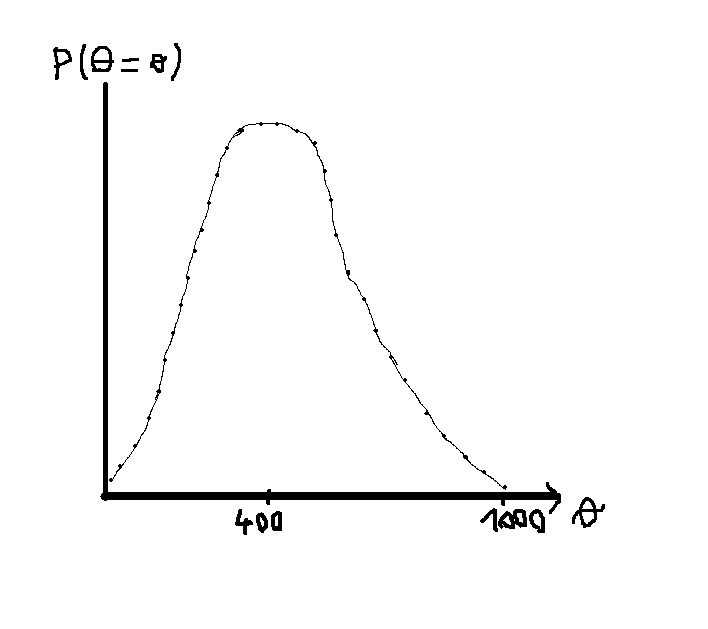
\includegraphics[scale=0.4]{apriori_1_1} \\
Privzamemo (kar!) $\Theta \sim B\left(1000, \frac{4}{10}\right)$ \\
$\implies P(\Theta = \theta) = \binom{1000}{\theta} \left(\frac{4}{10}\right)^{\theta} \left(1-\frac{4}{10}\right)^{1000-\theta}$. \\
$P(k$ črnih od $10$ izvlečenih$ \mid \Theta = \theta) = \frac{\binom{\theta}{k} \binom{1000-\theta}{10-k}}{\binom{10}{k}}$ (*) \\
(*) pri omejitvah ($k$ omejimo). \\
Osvežena porazdelitev - novo vedenje \\
\begin{align*}
  &P(\Theta = \theta \mid 6 \text{ črnih od } 10 \text{ izvlečenih}) = \\
  &\frac{P(6 \text{ črnih od } 10 \text{ izvlečenih} \mid \Theta = \theta) \cdot P(B(1000, \frac{4}{10}) = \theta)}
    {\sum_{i=0}^{1000} P(6 \text{ črnih od } 10 \text{ izvlečenih} \mid \Theta = i) \cdot P(B(1000, \frac{4}{10})) = i}.
\end{align*}
Pravimo ji aposteriorna porazdelitev.


\section{Proučevani slučajni vektor (vzročni) parametrični model}

Naj bo $X = (X_1, X_2 \dots X_n) \in \R^n$ preučevani slučajni vektor.
Pogosto so neodvisni in enako porazdeljeni (NEP) realizacija danega slučajnega eksperimenta.
S pomočjo statistike lahko \sn{ocenjujemo} porazdelitev slučajnega vektorja $X$.
Zanjo privzamemo, da pripada nekemu modelu, t.j. neki množici dopustnih rešitev.
Privzamemo, da je ta množica parametrizirana s parametričnim prostorom $\Theta \subset \R^r$.
Tu si mislimo, da parameter $\theta \in \Theta$ dobimo kot realizacijo slučajnega vektorja (s.v.) $\Theta$
z vrednostmi v $\Theta$ (večinoma $r \geq 2$).
Porazelitvi s.v. $X_i$ pogojno na $\Theta = \theta$ pravimo vzorčna porazdelitev.
Privzeli bomo, da imamo gostote $f(x \mid \theta)$ ali verjetnostne funkcije
\begin{equation*}
  P(X = x \mid \theta) = f(x \mid \theta),
\end{equation*}
torej da velja
\begin{equation*}
  P(X \in B \mid \Theta = \theta) = \int_B f(x \mid \theta) d\nu (x)
\end{equation*}
(v Lebesgueovi meri) ali
\begin{equation*}
  P(X \in B \mid \Theta = \theta) = \sum_{x \in B} f(x \mid \theta).
\end{equation*}
Modelu pogojnih porazdelitev $(X \mid \Theta = \theta)$ pravino vzorčni model.


\section{Apriorna in \sn{robna} porazdelitev}

Porazdelitvi fiktivnega slučajnega vektorja $\Theta$ pravimo apriorna porazdelitev,
brezpogojni (robni) porazdelitvni slučajnega vektorja $X$ pa pravimo \sn{robna} porazdelitev \\
(*) v resnici sta obe porazdelitvi robni porazdelitvi družne porazdelitve vektorja $(X, \Theta)$ z vrednostmi v $\R^{n+r}$.
\begin{exmp}
  Ocenjujemo Bernoullijevo porazdelitev. Predhodno vedenje je podano z apriorno prazdelitvijo na $(0,1)$;
  mislimo si, da je $p$ realizacija slučajne spremenljivke (s.s.) $\Pi$ z vrednostmi v $(0,1)$. Možnosti:
  \begin{itemize}
    \item nimamo apriornega mnenja o (dejanskem) $p$: tedaj bi (morda) vzeli zvezno porazdelitev z gostoto enakomerna porazdelitve, \\
      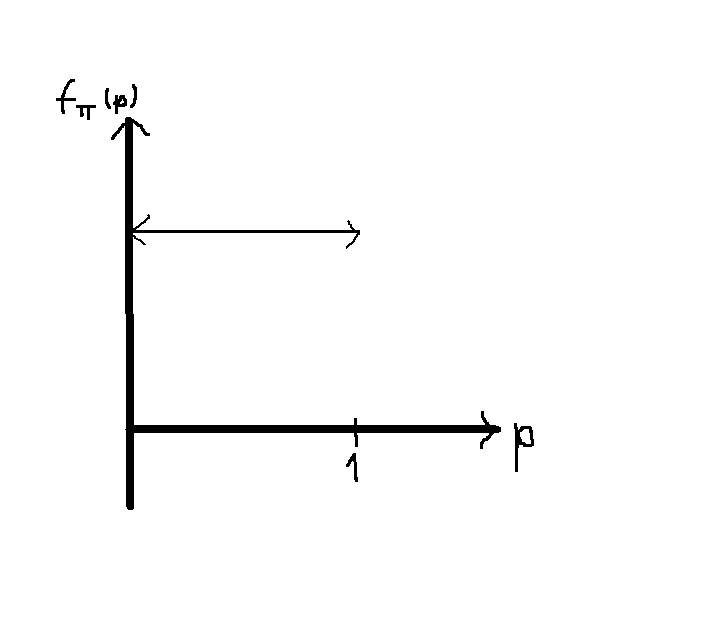
\includegraphics[scale=0.4]{apriori_nimamo_1_3} \\
    \item smo \sn{zelo} prepričani, da je (dejanski) $p \approx \frac{1}{2}$. \\ %Tedaj bi imeli
      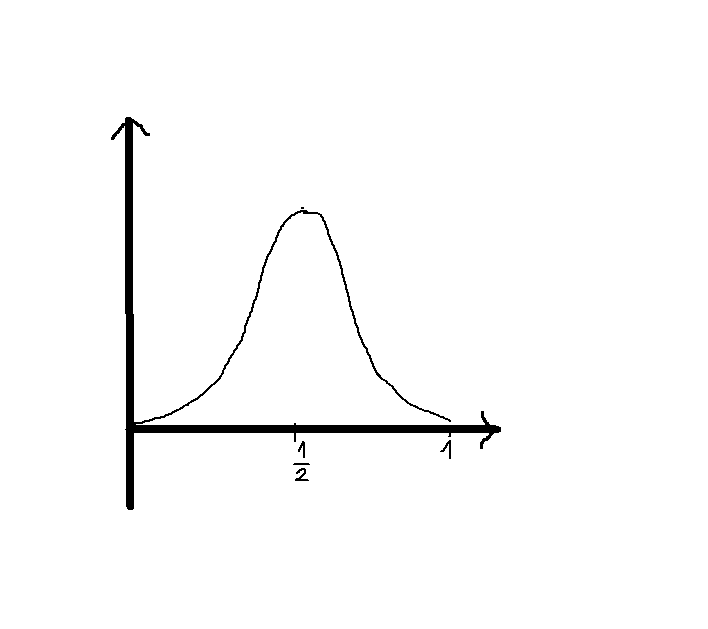
\includegraphics[scale=0.4]{apriori_imamo_1_3} \\
  \end{itemize}
\end{exmp}
Recimo, da je $f(p)$ gostota apriorne porazdelitve. Tedaj so apriorne verjetnosti
\begin{equation*}
  P(\Pi \in (a,b)) = \int_{a}^{b} f(p) dp
\end{equation*}
in apriorna pričakovana vrednost
\begin{equation*}
  E(\Pi) = \int_{0}^{1} p f(p) dp. 
\end{equation*}
Pripomnimo, da pri $\Pi \sim U(0,1)$ dobimo $E(U(0,1)) = \frac{1}{2}$. \\
Privzemimo, da smo \sn{vzorčili} $p$, potem pa \sn{neodvisno} $n$-krat vržemo $p$-kovanec ($P($cifra$=p)$),
gre za slučajne spremenljivke $X_1, X_2 \dots X_n$, za katere je $(X_i \mid \Pi = p) \sim Bernoulli(p)$
in so $X_1 \dots X_n$ neodvisne pogojno na $p$.
To ne pomeni, da do $X_1 \dots X_n$ brezpogojno neodvisne. \\
Za $i \neq j$ je
\begin{align*}
  P(X_i = 1 \land X_j = 1) &= \int_{0}^{1} P(X_i = 1 \land X_j = 1 \mid \Pi = p) f(p) dp = \\
  &\stackrel{\text{pogojno neodvisne}}{=}  \int_{0}^{1} P(X_i = 1 \mid \Pi = p) P(X_j = 1 \mid \Pi = p) f(p) dp = \\
  &= \int_{0}^{1} p^2 f(p) dp = \\
  &= E(\Pi^2).
\end{align*}
Ker je $P(X_i = 1) = \int_{0}^{1} P(X_i = 1 \mid p) f(p) dp = \int_{0}^{1} p f(p) dp = E(\Pi)$, je
\begin{equation*}
  Cov(X_i, X_j) = E(\Pi^2) - E(\Pi)^2 = D(\Pi)
\end{equation*}
za $i \neq j$, torej so $X_i$ brezpogojno neodvisne $\iff$ $\Pi =$ konstantna (slučajna spremenljivka). \\
Tvorimo $X = X_1 + \dots + X_n \in \{0, 1 \dots n\}$.
To je \sn{preučevana} slučajna spremenljivka.
Velja $(X\mid \Pi = p) \sim B(n,p)$.
To je vzorčna porazdelitev; vzročni model je parametriziran s prostorom parametrov $(0,1) = \Theta$.
Robna porazdelitev je podana z verjetnostmi
\begin{align*}
  P(X = k) &= \int_{0}^{1} P(X = k \mid p) f(p) dp = \\
  &= \int_{0}^{1} \binom{n}{k} p^k (1-p)^{n-k} f(p) dp.
\end{align*}
Recimo, da \sn{opazimo} $X = k$. Aposteriorna porazdelitev (osveženo vedenje o $p$) je sestavljeno iz verjetnosti
\begin{align*}
  P(X \in (a,b) \mid X = k) &= \frac{P(X = k \land \Pi \in (a,b))}{P(X = k)} = \\
  &= \frac{\int_{0}^{1} P(X = k \land \Pi \in (a,b) \mid \Pi = p) f(p) dp}{P(X = k)} = \\
  &= \int_{a}^{b} \frac{P(X = k \mid \Pi = p)}{P(X = k)} f(p) dp.
\end{align*}
Opazimo, da ima aposteriorna porazdelitev $(\Pi \mid X = k)$ gostoto
\begin{equation*}
  f_{(\pi \mid X)}(p \mid k) = \frac{P(X = k \mid p) f(p)}{P(X = k)}.
\end{equation*}
Zgornji formuli pravimo Bayesova formula. \\
Za številsko oceno za $p$ bi lahko vzeli pričakovano vrednost aposteriorne porazdelitve
\begin{equation*}
  \hat{p} = E(\Pi \mid X = k) = \int_{0}^{1} p \cdot f(p \mid k) dp.
\end{equation*}
Pravimo ji aposteriorna pričakovana vrednost. \\
Posebej priročna družina apriornih porazdelitev (za binomske vzorčne porazdelitve) je t.i.
$Beta = \{Beta(a,b) \mid a,b \in (0, \infty)\}$
\begin{equation*}
  f_{Beta(a,b)}(p) = \frac{1}{B(a,b)} p^{a-1} (1-p)^{b-1} 1_{(0,1)}(p)
\end{equation*}
(tu je $B(a,b) = \int_{0}^{1} p^{a-1} (1-p)^{b-1} dp$). \\
\begin{align*}
  &E(Beta(a,b)) = \frac{a}{a+b} \\
  &D(Beta(a,b)) = \frac{ab}{(a+b)^2 (a+b+1)}.
\end{align*}
$D(Beta(a,b))$ predstavlja \sn{težo} apriornega prepričanja; večji - manj sigurni smo. \\
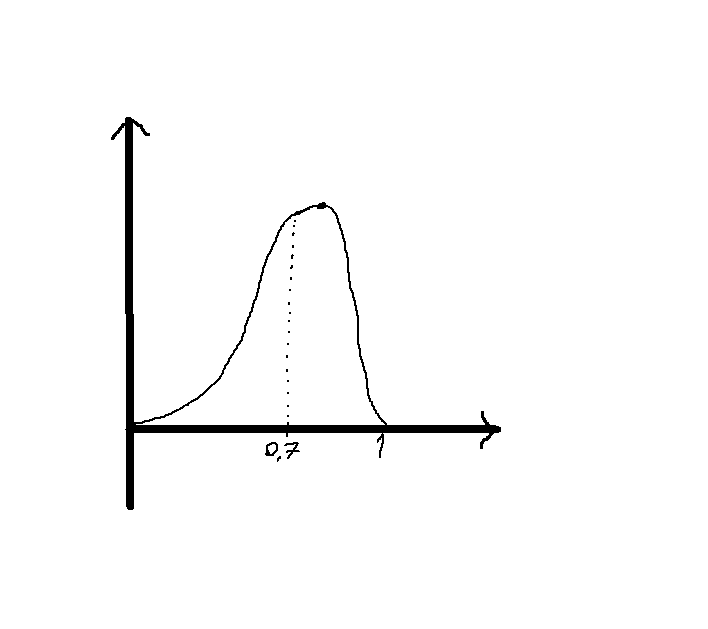
\includegraphics[scale=0.4]{aposteriori_1_4} \\
\begin{equation*}
  E(Beta(a,b)) = 0.7.
\end{equation*}
Aposteriorna porazdelitev ima gostoto (če je $f(p) = f_{Beta(a,b)}(p)$)
\begin{align*}
  f(p \mid k) &= \frac{\binom{n}{k} p^k (1-p)^{n-k} \cdot \frac{1}{B(a,b)} p^{a-1} (1-p)^{b-1}}{P(X = k)} = \\
  &= \text{konst.} \cdot p^{a+k-1} (1-p)^{b+n-k-1}.
\end{align*}
Vidimo, da je $(\Pi \mid X = k) \sim Beta(a+k, b+n-k)$. \\
Aposteriorna pričakovana vrednost (p.v.) je
\begin{align*}
  \frac{a+k}{a+b+n} &= \frac{(a+b)\frac{a}{a+b} + n \frac{k}{n}}{a+b+n} = \\
  &= \frac{a+b}{a+b+n} \cdot \frac{a}{a+b} + \frac{n}{a+b+n} \cdot \frac{k}{n}.
\end{align*}
Tukaj je
\begin{itemize}
  \item $\frac{a}{a+b}$ apriorna ocena,
  \item $\frac{k}{n}$ vzorčna ocena in
  \item $\frac{a+b}{a+b+n}$ in $\frac{n}{a+b+b}$ faktorja pri konveksni kombinaciji obeh ocen.
\end{itemize}
Vzorec velik $\to$ prevlada mnenje vzorca.


% 2. predavanje: 3.10.

\section{Disperzija aposteriornih porazdelitev}

Gre pravzaprav za disperzijo pogojnih porazdelitev.
Naj bosta $X: \Omega \to \R^m$ in $Y: \Omega \to \R^n$ in naj ima $(X,Y)$ gostoto $f_{(X,Y)}$ glede na $\mu \times \nu$
Sledita gostoti \\
$f_X(x) = \int f_{(X,Y)}(x,y) d\nu (y)$ za $X$ glede na $\mu$ in \\
$f_Y(y) = \int f_{(X,Y)}(x,y) d\mu (x)$ za $Y$ glede na $\nu$.
Dalje definiramo pogojni porazdelitvi $(Y \mid X = x)$ in $(X \mid Y = y)$ preko gostot
\begin{equation*}
  f_{(Y \mid X)}(y \mid x) = \frac{f_{(X,Y)}(X,Y)}{f_X(x)}
\end{equation*}
glede na $\nu$: gostota v $X \to \mu$ in simetrično za $f_{(X \mid Y)}(x \mid y)$. \\
$P(Y \in B) \mid X = x = \int_B f_{(Y \mid X)}(y \mid x) d\nu (y)$ - porazdelitev, opremljena z gostoto.
\begin{defn}
  \begin{equation*}
    E(Y \mid X = x) = \int y f_{(Y \mid X)}(y \mid x) d\nu (y).
  \end{equation*}
  $y$ lahko zamenjamo s $h(y)$. \\
  Pišemo $E(Y \mid X = x) = u(X)$ - $h$ je identiteta.
\end{defn}
\begin{defn}
  \begin{equation*}
    E(Y \mid X) = u(X): \Omega \to \R^n.
  \end{equation*}
  Slučajni vektor $\to$ pogojna pričakovana vrednost, \\
  oz.
  \begin{equation*}
    E(Y \mid X)(\omega) = u(X(\omega)) = E(Y \mid X = X(\omega)).
  \end{equation*}
  $E(Y \mid X)(\omega)$: funkcija na $X$, kompozitum. \\
  $X(\omega)$: vrednost.
\end{defn}
\begin{defn}
  Pogojno varianco slučajnega vektorja $Y$, pogojno na $X = x$ definiramo kot varianco pogojne porazdelitve $(Y \mid X = x)$, t.j.
  \begin{equation*}
    E((Y - u(X))(Y - u(X))^T \mid X = x) =: Var(Y \mid X = x).
  \end{equation*}
  Ker je $E$ aditivna, velja
  \begin{equation*}
    E((Y - u(X))(Y - u(X))^T \mid X = x) = E(Y Y^T \mid X = x) - u(X) u(X)^T =: v(X).
  \end{equation*}
  $v(X)$ je $n \times n$ matrika.
\end{defn}
\begin{defn}
  Pogojna varianca slučajnega vektorja $Y$ pogojno na slučajni vektor $X$ je
  \begin{equation*}
    Var(Y \mid X) = v(X).
  \end{equation*}
\end{defn}


% 3. predavanje: 9.10.

Zadnjič: beta-binomski model: proučevana s.s. $T$;
vzorčne porazdelitve $(T \mid p) \sim B(n,p)$ za $p \in \Theta = (0,1)$.
Če je apriorna porazdelitev $Beta(a,b)$, je aposteriorna pri $T = k$ enaka $Beta(a+k, b+n-k)$. \\
Disperzija porazdelitve $(\Pi \mid T = k)$ je enaka $\frac{(a-k)(b+n-k)}{(a+b+k)^2(a+b+n+1)}$
(in je odvisna od realizacije $k$). \\
DN: za katere $k$ je $D$(aposteriorne) $> D$(apriorne). \\
Izkaže se, da je za nekatere $k$ manjša, za nekatere $k$ pa večja od disperzije apriorne porazdelitve.
Vendar pa velja t.i. \sn{zakon popolne porazdelitve}
\begin{equation*}
  Var(\Theta) = E(Var(\Theta \mid X)) + Var(E(\Theta \mid X)),
\end{equation*}
kjer sta seveda
\begin{align*}
  &E(Var(\Theta \mid X)) \geq 0 \text{ in} \\
  &Var(E(\Theta \mid X)) \geq 0,
\end{align*}
($X$ vzorčni), iz katerega sledi $E(Var(\Pi \mid X)) \leq Var(\Theta)$ (apriori).
V konkretnem primeru je
\begin{equation*}
  E(Var(\Pi \mid T)) \leq Var(\Pi).
\end{equation*}
\begin{rem}
  \begin{equation*}
    E(Var(\Pi \mid T)) = \sum_{k=0}^{n} Var(\Pi \mid k) \cdot P(T = k);
  \end{equation*}
  $T$ vzorčimo, $T$ je robna porazdelitev (binomska pogojna?).
\end{rem}
(V povprečju aposteriorna varianca boljša.)


\section{Aposteriorni kredibilnostni interval}

(Bayesova različica intervala zaupanja). \\
V konkretnem zgledu \sn{iščemo} funkciji realizacije $L(k), U(k)$, za kateri velja
\begin{equation*}
  \forall k \; P\left(L(k) \leq p \leq U(k)\right) \geq 1-\alpha.
\end{equation*}
$p$ je slučajen. \\
Ker za $\Pi \sim Beta(a,b)$, vemo $(\Pi \mid T=k) \sim Beta(a+k, b+n-k)$, lahko izberemo
\begin{align*}
  &L(k) = F_{Beta(a+k,b+n-k)}^{-1}\left(\frac{\alpha}{2}\right), \\
  &U(k) = F_{Beta(a+k,b+n-k)}^{-1}\left(1 - \frac{\alpha}{2}\right)
\end{align*}
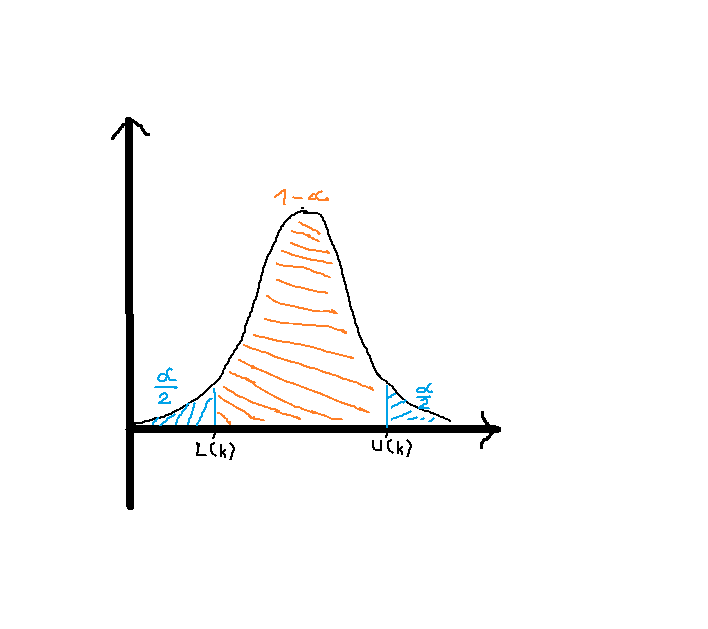
\includegraphics[scale=0.5]{interval_kvantili_1_5} \\
in v aposteriorni kredibilnostni interval (AKI) dobimo $= 1 - \alpha$.
Taki konstrukciji pravimo centralni kredibilnostni interval.
V praksi pogosto uporabljamo tudi t.i. kredibilnostni interval največje gostote, kjer zahtevamo
\begin{equation*}
  f_{(\Pi \mid T=k)}(L(k)) = f_{(\Pi \mid T=k)}(U(k)).
\end{equation*}
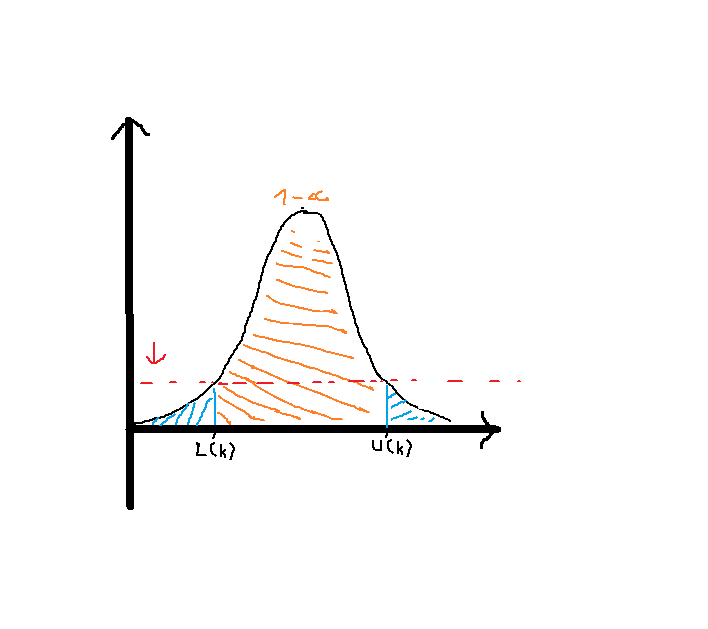
\includegraphics[scale=0.5]{interval_kredibilnostni_1_5} \\
To ima smisel za unimodalne aposteriorne porazdelitve.


\section{Splošne oznake}

$X$ - proučevalni vektor (z vrednostmi v $\R^n$). \\
$x$ - realizacija vektorja $X (x \in \R^n)$. \\
$\Theta \subset \R^n$ - parametrični prostor. \\
$\Theta$ - (fiktivni) vektor z realizacijo $\theta \in \Theta$. \\
$P = \{P_{\theta} = (X \mid \Pi = \theta) \mid \theta \in \Theta\}$ - družina vzorčnih porazdelitev (vzorčni model). \\
$f(x \mid \theta)$ - gostota (ali verjetnostna funkcija) porazdelitve $(X \mid \Theta = \theta)$
(izračunano v $x$). \\
\begin{rem}
  $f(x \mid \theta) = f_{X \mid \Theta}(x \mid \theta)$ - spuščamo.
\end{rem}
V istem smislu gostota (ali verjetnostna funkcija) apriorne porazdelitve.
Za aposteriorno gostoto (ali verjetnostno funkcijo) velja Bayesova formula (BF)
\begin{equation*}
  f(\theta \mid x) = \frac{f(x \mid \theta) f(\theta)}{f(\theta)} \propto f(x \mid \theta) f(\theta).
\end{equation*}
$f(x)$ je normalizacijski faktor.



\chapter{Enoparametrični modeli}


\section{Beta-binomski model}

Uvodni beta-binomski model je enoparametričen.


\section{Poissonov model (gama-poissonov model)}

Naj bo parametrični prostor $\Theta = (0, \infty)$ in naj bo $X = (X_1 \dots X_n)$,
kjer so $(X_i \mid \lambda) \stackrel{\text{NEP}}{\sim} Poisson(\lambda)$.
Za proučevano s.s. vzamemo $T = \sum_{i=1}^{n} X_i$; seveda je $(T \mid \lambda) \sim Poisson(n\lambda)$. \\
Privzemimo apriorno porazdelitev
\begin{equation*}
  f(\lambda) = f_{Gama(a,b)}(\lambda) = \frac{b^a}{\Gamma(a)} \lambda^{a-1} e^{-b\lambda} \cdot 1_{(0,\infty)}(\lambda).
\end{equation*}
$(0,\infty)$ je parametrični prostor, $a$ in $b$ sta pozitivni konstanti. \\
Izkaže se:
\begin{align*}
  &E(Gama(a,b)) = \frac{a}{b}, \\
  &D(Gama(a,b)) = \frac{a}{b^2}.
\end{align*}
DN. \\
\begin{equation*}
  P(T = k \mid \lambda) = e^{-n \lambda} \frac{(n \lambda)^k}{k!}.
\end{equation*}
Bayesova formula se glasi
\begin{align*}
  f(\lambda \mid T = k) &\propto P(T = k \mid \lambda) \cdot f(\lambda) \\
  &\propto e^{-n \lambda} \lambda^k \cdot \lambda^{a-1} e^{-b \lambda} \\
  &= \lambda^{a+k-1} e^{-(b+n) \lambda}
\end{align*}
$\implies (\Lambda \mid T = k) \sim Gama(a+k, b+n)$.

\begin{defn}
  Naj bo podan vzorčni model $P$ in naj bo $K$ družina porazdelitev na parametričnem prostoru $\Theta$.
  Pravimo, da je $K$ konjugirana k $P$, če vedno velja
  \begin{equation*}
    f(\theta \mid x) \in K \; \implies \; \forall x: \; (\Theta \mid X = x) \in K.
  \end{equation*}
  $f(\theta \mid x)$ je porazdelitev na $\Theta$.
  Rečemo lahko tudi, da sta $P$ in $K$ konjugiran par.
\end{defn}


\section{Normalni model z znano disperzijo}

Tu je $\sigma^2$ znana disperzija, vzorec $X = (X_1 \dots X_n)$ pa zadošča \\
$(X_i \mid \mu) \stackrel{\text{NEP}}{\sim} N(\mu, \sigma^2)$, kjer je $\mu \in \Theta = \R$.
S katero porazdelitvijo bi zakodirali apriorno informacijo? \\
Recimo, da je apriorno mnenje: $\mu \approx \mu_0$.
Vzemimo za apriorno porazdelitev kar $N(\mu_0, \tau_0^2)$. \\
Vzorčna:
\begin{align*}
  f(x \mid \mu) &= f(x_1 \dots x_n \mid \mu) \\
  &= (2 \pi \sigma^2)^{-\frac{1}{2}} e^{-\frac{1}{2 \sigma^2} \sum_{i=1}^{n} (x_i - \mu)^2}.
\end{align*}
Pripomnimo, da je
\begin{equation*}
  \sum_{i=1}^{n} (x_i - \mu)^2 = n \cdot (\mu - \overline{x})^2 + \sum_{i=1}^{n} (x_i - \overline{x})^2,
\end{equation*}
kjer je $\overline{x} = \frac{1}{n} \sum_{i=1}^{n} x_i$. \\
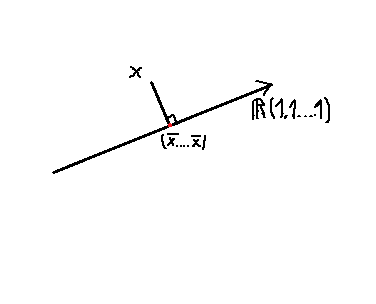
\includegraphics[scale=0.5]{x_prostorska_2_2} \\
$\R(1,1 \dots 1)$ - prostorska diagonala. \\
(Vzorčna: jih je več, apriorna: ena.) \\
Apriorna:
\begin{equation*}
  f(\mu) = (2 \pi \sigma_0^2)^{-\frac{1}{2}} e^{-\frac{1}{2 \sigma_0^2} (\mu - \mu_0)^2}.
\end{equation*}
Opazimo, da je
\begin{equation*}
  f(\mu) = e^{\text{kvadratni polinom}(\mu)}.
\end{equation*}
Velja:
\begin{equation*}
  \int_{-\infty}^{\infty} e^{a \mu^2 + b \mu + c} d\mu < \infty \; \iff \; a < 0.
\end{equation*}
DN (kako se narobe lotiti): drugače koliko apriorna gostota (integral robne gostote, Bayesova formula). \\
V tem duhu
\begin{equation*}
  f(\mu \mid x) \propto e^{-\frac{1}{2} \left(\left(\frac{n}{\sigma^2} + \frac{1}{\tau_0^2}\right) \mu^2 -
  2 \left(\frac{n \overline{x}}{\sigma^2} - \frac{\mu_0}{\tau_0^2}\right) \mu\right)}.
\end{equation*}
Prepoznamo kot normalno porazdelitev.
Označimo jo $N(\mu_1, \tau_1^2)$. \\
Velja
\begin{equation*}
  f_{N(\mu_1, \tau_1^2)}(\mu) \propto e^{-\frac{1}{2} \left(\frac{1}{\tau_1^2} \mu^2 - 2 \frac{\mu_2}{\tau_1^2} \mu\right)}.
\end{equation*}
Sledi
\begin{align*}
  &[\mu^2]: \; \frac{n}{\sigma^2} + \frac{1}{\tau_0^2} = \frac{1}{\tau_1^2} \text{ in} \\
  &[\mu]: \; \frac{n \overline{x}}{\sigma^2} + \frac{\mu_0}{\tau_0^2} = \frac{\mu_1}{\tau_1^2}.
\end{align*}
Tukaj je:
\begin{itemize}
  \item $\frac{n}{\sigma^2}$ vzorčna preciznost,
  \item $\frac{1}{\tau_0^2}$ apriorna preciznost,
  \item $\frac{1}{\tau_1^2}$ aposteriorna preciznost,
  \item preciznosti se pri seštevanju neodvisnih normalnih porazdelitvah seštevajo.
\end{itemize}
Preciznost je $\frac{1}{D(..)}$. \\
To pomeni
\begin{equation*}
  \tau_1^2 = (\frac{n}{\sigma^2} + \frac{1}{\tau_0^2})^{-1}
\end{equation*}
in
\begin{align*}
  \mu_1^2 &= \tau_1^2 (\frac{n}{\sigma^2} + \frac{1}{\tau_0^2}) \\
  &= \frac{(\frac{n}{\sigma^2} \overline{x} + \frac{1}{\tau_0^2} \mu_0) \cdot \frac{\tau_0^2 \sigma^2}{n}}
    {(\frac{n}{\sigma^2} + \frac{1}{\tau_1^2}) \cdot \frac{\tau_0^2 \sigma^2}{n}} \\
  &= \frac{\tau_0^2 \overline{x} + \frac{\sigma^2 \mu_0}{n}}{\tau_0^2 + \frac{\sigma^2}{n}} \\
  &= \frac{\tau_0^2}{\tau_0^2 + \frac{\sigma^2}{n}} \overline{x} +
    \frac{\frac{\sigma^2}{n}}{\tau_0^2 + \frac{\sigma^2}{n}} \mu_0
\end{align*}


\section{Eksponentne družine porazdelitev}

Vzorčni model pripada eksponentni družini porazdelitev, če velja
\begin{align}
  f(x \mid \theta) &= c(\theta) \cdot e^{\langle Q(\theta), T(x)\rangle} \cdot h(x) \nonumber \\
  &= e^{-\psi(\theta)} e^{\langle Q(\theta), T(x)\rangle} \cdot h(x), \label{eksponentna-osnova}
\end{align}
kjer je
\begin{align*}
  &\tau: \Theta \to \R \\
  &T: \R^n \to \R^m \\
  &Q: \Theta \to \R^m \text{ in} \\
  &h: \R^n \to [0, \infty].
\end{align*}
\begin{exmp}
  \begin{enumerate}[label=\protect\circled{\arabic*}] \text{}
    \item NEP Bernoullijev model: \\
      \begin{align*}
        &(X_i \mid p) \stackrel{\text{NEP}}{\sim} Bernoulli(p) = B(1,p) \\
        &f(x_1 \dots x_n \mid p) = p^{\sum_{i=1}^{n} x_i} (1-p)^{n-\sum_{i=1}^{n} x_i} \cdot 1_{\{0,1\}^n} (x_1 \dots x_n)
      \end{align*}
      % 1_{\{0,1\}^n} (x_1 \dots x_n) realizacija?
      \begin{equation*}
        f(x_1 \dots x_n \mid p) = P(X_1 = x_1 \dots X_n = x_n \mid p)
      \end{equation*}
      Preoblikujemo v:
      \begin{equation*}
        (1-p)^{n} \left(\frac{p}{1-p}\right)^{\sum_{i=1}^{n} x_i} \cdot 1_{\{0,1\}^n} (x_1 \dots x_n) =
        e^{\ln(\frac{p}{1-p}) \sum_{i=1}^{n} x_i} \cdot 1_{\{0,1\}^n} (x_1 \dots x_n).
      \end{equation*}
      
    \item Normalni model z znano $\sigma^2$: \\
      $\Theta = \R, \mu \in \R$
      \begin{align*}
        (EXP) \; f(x_1 \dots x_n \mid \mu) &= (2 \pi \sigma^2)^{-\frac{n}{2}} e^{-\frac{1}{2 \sigma^2} \sum_{i=1}^{n} (x_i - \mu)^2} \\
        &= (2 \pi \sigma^2)^{-\frac{n}{2}} e^{-\frac{1}{2 \sigma^2} \sum_{i=1}^{n} x_i^2
          + \frac{\mu}{\sigma^2} \sum_{i=1}^{n} x_i - \frac{n \mu^2}{2 \sigma^2}} \\
        &= (2 \pi \sigma^2)^{-\frac{n}{2}} \cdot e^{-\frac{n \mu^2}{2 \sigma^2}}
          \cdot e^{\frac{\mu}{\sigma^2} \sum_{i=1}^{n} x_i} \cdot e^{-\frac{1}{2 \sigma^2} \sum_{i=1}^{n} x_i^2}.
      \end{align*}
      Tukaj je
      \begin{align*}
        &c(\mu) = (2 \pi \sigma^2)^{-\frac{n}{2}} \cdot e^{-\frac{n \mu^2}{2 \sigma^2}} \\
        &Q(\mu) = e^{-\frac{\mu}{\sigma^2}} \\
        &T(x) = e^{\sum_{i=1}^{n} x_i} \\
        &h(x) = e^{-\frac{1}{2 \sigma^2} \sum_{i=1}^{n} x_i^2}
      \end{align*}
    \item Normalni model z neznano disperzijo: \\
      $\Theta = \R \times (0, \infty) = (\mu, \sigma^2)$ \\
      Zapišemo
      \begin{equation*}
        f(x_1 \dots x_n \mid \mu, \sigma^2) = (2 \pi \sigma^2)^{-\frac{n}{2}} e^{-\frac{n \mu^2}{2 \sigma^2}}
          e^{\left\langle \left(\frac{\mu}{\sigma^2}, -\frac{1}{2 \sigma^2}\right),
          \left(\sum_{i=1}^{n} x_i, \sum_{i=1}^{n} x_i^2\right)\right\rangle}.
      \end{equation*}
      Tukaj je
      \begin{align*}
        &c(\mu) = (2 \pi \sigma^2)^{-\frac{n}{2}} e^{-\frac{n \mu^2}{2 \sigma^2}} \\
        &Q(\mu) = \left(\frac{\mu}{\sigma^2}, -\frac{1}{2 \sigma^2}\right) \\
        &T(x) = \left(\sum_{i=1}^{n} x_i, \sum_{i=1}^{n} x_i^2\right).
      \end{align*}
      $m = 2$. \\
      Preimenujemo (EXP) in definirajmo apriorne gostote
      \begin{equation}
        \label{apriori-nornalna-neznana}
        f(\eta, \upsilon) = \frac{1}{K(\eta, \upsilon)} \cdot e^{\langle Q(\theta), \eta  \rangle - \upsilon \psi(\theta)}.
      \end{equation}
      Tukaj je $\mu \in \R^n$ in $\upsilon \in \R$. \\
      (Upoštevati moramo morebitne omejitve zaradi zahteve $\int F = 1$). \\
      Seveda je
      \begin{equation*}
        K(\eta, \upsilon) = \int e^{\langle Q(\theta), \upsilon \rangle - \upsilon \psi(\theta)} d\theta.
      \end{equation*}
      Aposteriorna gostota?
      \begin{equation*}
        f(\theta \mid x) \propto e^{-(\upsilon + 1) \psi(\theta) + \langle Q(\theta), \eta + T(x) \rangle}
      \end{equation*}
      Tukaj smo zmožili nekonstantne faktorje iz \ref{eksponentna-osnova} in \ref{apriori-nornalna-neznana}. \\
      Vidimo:
      \begin{equation*}
        f(\theta \mid x) = f_{(\eta + T(x), \upsilon + 1)}(\theta).
      \end{equation*}
      Gre za konjugirano družino.
      \begin{exmp}
        Aplicirajmo to konstrukcijo na modelu \circled{2}.
        Dobimo konjugirano družino
        \begin{equation*}
          f_{(\eta, \upsilon)}(\mu) \propto e^{\frac{\mu}{\sigma^2 \eta} - \tau \frac{n \mu^2}{2 \sigma^2}},
        \end{equation*}
        kjer sta $\eta, \upsilon \in \R$. \\
        Vidimo, da mora biti $\upsilon > 0$. \\
        DN: $\eta, \upsilon \to \mu_0, \tau_0^2$ - reparametrizacija.
      \end{exmp}
  \end{enumerate}
\end{exmp}


% 4. predavanje: 17.10.

\section{Neinformirane apriorne porazdelitve}

Neinformirana apriorna porazdelitev je taka, ki \sn{ne vsebuje predhodne informacije} o parametru.
Tovrsten koncept je šibko-informativna apriorna porazdelitev. % sovrsten?
Izkaže se, da s statistični praksi (tudi v aplikacija frekventistične statistike) potrebujemo ta koncept.

\begin{exmp}
  V Beta-binomskem modelu (..) je Laplace predlagal $U(0,1) = Beta(1,1)$ kot neinformirano porazdelitev. \\
  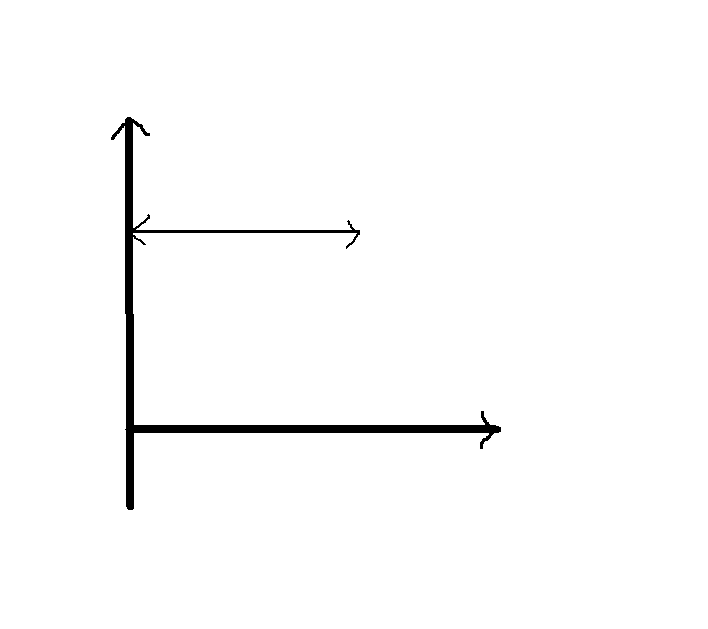
\includegraphics[scale=0.3]{ploščata_2_6} \\
  \sn{Ploščata porazdelitev}. \\
  \underline{Učinek reparametrizacije}
  \begin{exmp}
    Binomski vzorčni model: $f(k \mid p) = \binom{n}{k} p^k (1-p)^{n-k}, \; p \in (0,1)$. \\
    Reparametrizirajmo s parametrom $q = \ln\left(\frac{p}{1-p}\right) = logit(p)$.
    Dobimo
    \begin{align*}
      \widetilde{f}(k \mid q) &= f(k \mid logit^{-1}(q)) \\
      &= f\left(k \mid \frac{e^q}{1+e^q}\right) \\
      &= \binom{n}{k} \left(\frac{e^q}{1+e^q}\right)^k \left(\frac{1}{1+e^q}\right)^{n-k} \\
      &= \binom{n}{k} (1+e^q)^{-k} e^{kq} \quad (q \in \R).
    \end{align*}
    Kako je s transformacijo apriorne porazdelitve? \\
    Naj bo $\Pi$ slučajna spremenljivka z realizacijo $p$ in $Q$ slučajna spremenljivka z realizacijo $q$;
    velja $Q = logit \circ \Pi = logit(\Pi)$:
    \begin{align*}
      &f_Q(q) = f_{logit(\Pi)}(q) = f_{\Pi}(logit^{-1}(q)) \cdot \left|\frac{d}{dq} logit^{-1}(q)\right| \\
      &logit^{-1}(q) = 1 - \frac{1}{1+e^q} \implies \frac{d}{dq} logit^{-1}(q) = (1+e^q)^{-2} e^q.
    \end{align*}
    Sledi: če je $\Pi \in (0,1)$, je
    \begin{equation*}
      f_Q(q) = \frac{e^q}{(1+e^q)^2};
    \end{equation*}
    ali je to še ploščata porazdelitev? \\
    Jeffreys je kot privzeto neinformativno porazdelitev predlagal
    \begin{equation}
      \label{Jeffrey-neinformativna}
      f(\theta) \propto \sqrt{|det (FI(\theta))|}.
    \end{equation}
    Tu je $FI(\theta)$ t.i. Fisherjeva informacija:
    \begin{align*}
      FI(\theta) &= E_{(X \mid \Theta)} (grad_{\theta} \ln(f(x \mid \theta)) \cdot grad_{\theta} \ln(f(x \mid \theta))^T) \\
      &= Var_{(X \mid \Theta)} (grad_{\theta} \ln (f(x \mid \theta))) \\
      &= -E_{(X \mid \Theta)} (H_{\theta} (ln f) (x \mid \theta)).
    \end{align*}
    Za $\theta \in \Theta \subset \R^r$ je $grad_{\theta} \ln (f(x \mid \theta))$ vektor s komponentami
    $\frac{\partial}{\partial \theta_i} \ln(f(x \mid \theta))$ za $1 \leq i \leq r$.
  \end{exmp}
  \underline{Učinek reparametrizacije na Jeffreysovo apriorno porazdelitev} \\
  Reparametrizirajmo s parametrom $\lambda = \phi(\theta)$, kjer je
  \begin{equation*}
    \phi: \Theta \subset \R^n \to \Lambda \subset \R^n
  \end{equation*}
  diferenciabilen; sledi
  \begin{equation*}
    \widetilde{f}(x \mid \lambda) = f(x \mid \phi^{-1}(\lambda)).
  \end{equation*}
  Odvajajmo
  \begin{align*}
    \frac{\partial}{\partial \lambda_i} \ln(\widetilde{f}(x \mid \lambda)) &=
      \sum_{j=1}^{n} (\frac{\partial}{\partial \lambda_j} \ln(f(x \mid \lambda_j)) \cdot
        \frac{\partial (\psi^{-1})_j}{\partial \lambda_i} (\lambda)) \\
    &= \left[\frac{\partial (\psi^{-1})_j}{\partial \lambda_i}\right]_{j=1}^n
      \cdot grad_{\theta} (\ln f) (x \mid \phi^{-1}(\lambda))
  \end{align*}
  \begin{equation*}
    grad_{\lambda} f(x \mid \lambda) = [J(\phi^{-1}(\lambda))]^T \cdot grad_{\theta} \ln f (x \mid \phi^{-1}(\lambda))
  \end{equation*}
  $J$: Jacobijeva matrika.
  \begin{align*}
    \ln \widetilde{f}(x \mid \lambda) &= \ln(f(x \mid \phi^{-1}(\lambda))) \cdot
      grad_{\lambda} \ln(f(x \mid \lambda)) \cdot grad_{\lambda} \ln(f(x \mid \lambda))^T \\
    &= [J \phi^{-1}(\lambda)]^T \cdot grad_{\theta} \ln f (x \mid \phi^{-1}(\lambda)) \cdot
      grad_{\theta} \ln f (x \mid \phi^{-1}(\lambda))^T \cdot [J \phi^{-1}(\lambda)] \\
    &\implies \widetilde{FI}(\lambda) = (J \phi^{-1}(\lambda))^T \cdot
      FI(\phi^{-1}(\lambda)) \cdot J \phi^{-1}(\lambda).      
  \end{align*}
  Kaj je Jeffreysova apriorna porazdelitev na $\lambda$?
  \begin{align*}
    &f_{Jeffrey}(\lambda) = c \sqrt{det \widetilde{FI}(\lambda)} = \\
    &= c \sqrt{det FI (\phi^{-1}(\lambda))} = c |det J(\phi^{-1}(\lambda))|;
  \end{align*}
  to je transformirana Jeffreysova apriorna porazdelitev (transformirana sama vase).
\end{exmp}


% 5. predavanje: 23.10.

\chapter{Monte-Carlo integracija in metode vzorčenja}


Proučujemo (neznani) parameter vzorčnega povprečja, recimo da nas zanima realnoštevilska funkcija $h(\theta)$.
\begin{exmp} \text{} \\
  Morda nas zanima \sn{$E(X^2)$} naše preučevane slučajne spremenljivke.
  Če imamo normalni model s parametrom $\theta = (\mu, \sigma^2)$, nas torej zanima $h(\mu, \sigma^2) = (\mu^2, \sigma^2)$.
  V Bayesovem okviru iz apriorne porazdelitve in vzorca dobimo aposteriorno porazdelitev z gostoto
  \begin{equation*}
    f(\theta \mid x) = \frac{f(x \mid \theta) f(\theta)}{f(x)},
  \end{equation*}
  kot oceno za $h(\theta)$ vzamemo npr. aposteriorno pričakovano vrednost
  \begin{equation*}
    E(h(\theta) \mid X = x) = \int h(\theta) f(\theta \mid x) d\theta.
  \end{equation*}
\end{exmp}
Problemi:
\begin{itemize}
  \item $h(\theta) f(\theta \mid x)$ je lahko zahtevna za integracijo - numerično,
  \item morda je \sn{že} $f(x \mid \theta) f(\theta)$ zahtevna za integracijo in $f(x)$ sploh ne \sn{poznamo}.
\end{itemize}
Odgovor na to je integracija Monte-Carlo z Markovskimi verigami.


\section{Klasična integracija Monte-Carlo}

\begin{exmp}
  \sn{Integrirajte} $\int_{0}^{1} \left| \sin(100 \sin(\pi x))\right| dx$.
\end{exmp}
Spomnimo se na KZVŠ: če so $X_1, X_2 \dots$ NEP slučajni vektorji s pričakovano vrednostjo $\mu$, velja
\begin{equation*}
  \frac{x_1 + \dots + x_n}{n} \to \mu = \int x f(x) dx
\end{equation*}
skoraj gotovo (s.g.). \\
Če je $h$ taka realnoštevilska funkcija, da obstaja $E(h(X_i))$,
so tudi $h(X_1), h(X_2) \dots$ NEP s pričakovano vrednostjo $E(h(X_i))$ in zato
\begin{equation*}
  \frac{h(x_1) + \dots + h(x_n)}{n} \to E(h(X_i)) = \int h(x) f(x) dx
\end{equation*}
skoraj gotovo. \\
S pomočjo KZVŠ lahko ocenimo integral dane funkcije $h: (0,1) \to \R$ na naslednji način:
privzamemo zaporedje NEP $X_i \sim N(0,1)$, torej velja
\begin{equation*}
  \frac{h(x_1) + \dots + h(x_n)}{n} \to \int h(x) .|. dx
\end{equation*}
skoraj gotovo. \\
Kaj to pomeni? \\
Verjetnost tistih zaporedij $(X_1, X_2 \dots)$,
pri katerih limita $\frac{1}{n} \sum_{i=1}^{n} h(x_i)$ obstaja in je enaka $.|.$. \\
Tu manjka ocena za natančnost ocene. \\
DN: implementirajmo. \\
NEP - izziv. \\
Izkaže se, da s psevdonaključnimi števili znamo izvrstno simulirati NEP.
Vzorčenje iz $(0,1)$ (za razumno velike vzorce). \\
Oceno natančnosti lahko dobimo s pomočjo CLI: privzemino obstoj disperzije slučajne spremenljivke $X_i$
($\iff \int h(x)^2 f(x) dx < \infty$).
\begin{equation*}
  S^2 = \frac{1}{n-1} \sum_{i=1}^{n} (h(X_i) - \overline{h(X_i)})^2.
\end{equation*}
Po CLI velja
\begin{equation*}
  \frac{h(X_i) - E(h(X_i))}{\frac{S}{\sqrt{n}}} \xrightarrow[n \to \infty]{D} N(0,1).
\end{equation*}
Za $\alpha \in (0, \frac{1}{2})$ sledi
\begin{equation*}
  P\left(\frac{\overline{h(X_i)} - E(h(X_i))}{\frac{S}{\sqrt{n}}} \in [-z_{\frac{\alpha}{2}}, z_{\frac{\alpha}{2}}]\right) = 1 - \alpha%\to
\end{equation*}
Verjamemo, da se ocena $\overline{h(x_i)}$ razlikuje od dejanskega integrala $E(h(x_i))$ za kvečjemu
$z_{\frac{\alpha}{2}} \cdot \frac{s}{\sqrt{n}}$.


% 6. predavanje: 24.10.

\section{Simulacija vzorčenja z inverzno kumulativno porazdelitveno funkcijo}

Privzemimo, da je \sn{ciljna} kumulativna porazdelitvena funkcija (k.p.f.) \\
$F: \R \to [0,1]$ zvezna bijekcija $\R \to (0,1)$.
Velja trditev.
\begin{claim}
  Naj bo $U \sim U(0,1)$. Tedaj je $F^{-1}(U) \sim F$.
\end{claim}
\begin{conseq}
  Če \sn{poznamo} $F^{-1}$, znamo simulirati vzorčenje \sn{iz $F$}.
\end{conseq}
\begin{pro}
  $P(F^{-1}(U) \leq x) = P(U \leq F(x)) = F(x)$.
\end{pro}
\begin{exmp}
  \sn{Poznamo} $\Phi^{-1}$, kjer je $\Phi(x) = \int_{-\infty}^{x} \frac{1}{\sqrt{2\pi}} e^{-\frac{t^2}{2}} dt$.
\end{exmp}
Zgornja trditev je standardna metoda za vzorčenje iz $N(0,1)$
($\stackrel{\text{vaja}}{\implies}$ znamo vzorčiti iz $N(\mu, \Sigma)$ za poljubne $\mu \in \R^d$ in $\sigma \in \R^{d \times d}$ s.p.d.). \\
V splošnem, če definiramo posplošeni inverz
\begin{equation*}
  F^{-}(U) = \inf F^{-1}([u, \infty)),
\end{equation*}
je (še vedno) $F^{-1}(U) \sim F$. ($\stackrel{\text{vaja}}{\implies}$ znamo vzorčiti iz končnih diskretnih porazdelitev).


\section{Metoda sprejmi ali zavrni (A/R)}

\underline{Motivacija:} Naj bo $f: \R \to [0, \infty)$ ciljna (Lebesgueova) gostota.
Označimo \sn{graf} pod njo:
\begin{equation*}
  A_f = \{(x, u) \mid 0 \leq u \leq f(x)\} \subset \R^2.
\end{equation*}
Seveda je $S(A_f) = 1$ (ploščina). \\
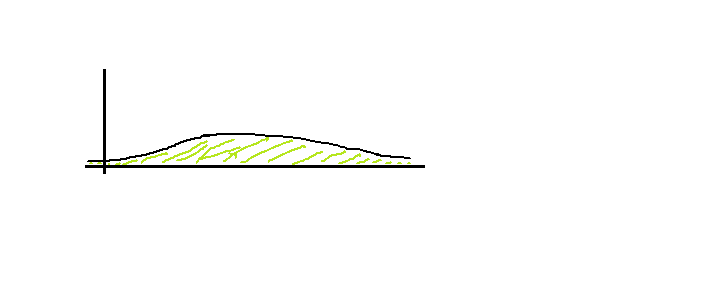
\includegraphics[scale=0.4]{območje_3_3} \\
Pripomnimo, da za $(X,U) \sim U(A_f)$ velja $X \sim f$:
\begin{equation*}
  f_X(x) = \int_{u=-\infty}^{\infty} f_{(X,U)}(x,u) du = \int_{0}^{f(x)} du = f(x).
\end{equation*}
\begin{enumerate}[label={A/R \#\arabic{*}:}]
  \item privzemimo $\{x \mid f(x) > 0\} \subset (a,b)$, kjer $-\infty < a < b < \infty$ in $\exists m: f(x) < m$ za vse $x$. \\
    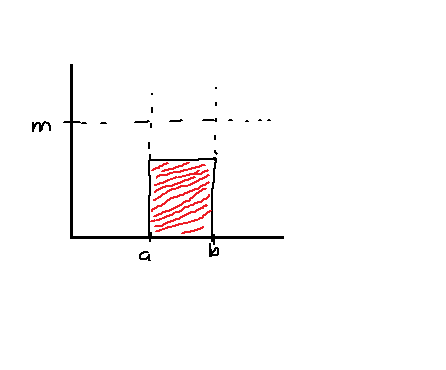
\includegraphics[scale=0.5]{meja_območje_3_3} \\
    Simulacijo vzorčenja $X \sim f$ implementiramo takole:
    \begin{enumerate}[label=(\roman*)]
      \item vzorčimo $Y=y$, kjer $Y \sim (a,b)$ -\sn{$x$},
      \item vzorčimo $(V \mid Y=y) = v$ (realizacija) iz $U(0,m)$ -\sn{$y$},
      \item če je $v < f(y)$ sprejmemo $X=y$, če je $v \geq f(y)$ zavrnemo $y$ in ponovimo (i).
    \end{enumerate}
    Preverimo $X \sim f$. Za $I \subset (a,b)$ je
    \begin{align*}
      P(X \in I) &\stackrel{\text{vaja}}{=} P(Y \in I \mid v < f(y)) \\
      &= \frac{\int_{\R} P(Y \in I \land v < f(Y) \mid Y=y) \cdot f_Y(y) dy}
        {\int_{\R} P(v < f(Y) \mid Y=y) \cdot f_Y(y) dy} \\
      &\stackrel{\text{pogojna}}{=} \frac{\int_{\R} P(y \in I \land v < f(y)) \cdot f_Y(y) dy}
        {\int_{\R} P(v < f(y)) \cdot f_Y(y) dy} \\
      &\stackrel{I \subset (a,b)}{=} \frac{\int_{I} P(v < f(y)) \cdot \frac{1}{b-a} dy}
        {\int_{(a,b)} P(v < f(y)) \cdot \frac{1}{b-a} dy} \\
      &= \frac{\int_{I} f(y) dy}
        {\int_{(a,b)} f(y) dy} \\
      &= \int_I f(y) dy,
    \end{align*}
    kjer smo v zadnjem koraku upoštevali $P(V < f(y)) = \frac{f(y)}{m}$ na $(a,b)$. \\ % in da je V enakomerno porazdeljena
    $\int_I f(y) dy$ je gostota $X$.
  \item Privzemimo, da znamo vzorčiti iz gostote $g: \R \to [0,\infty)$ in da je $f(x) < M \cdot g(x)$ za vse $x$ (za neki $M$).
    Simulacijo vzorčenja $X \sim f$ implementiramo takole:
    \begin{enumerate}[label=(\roman*)]
      \item vzorčimo $Y=y$, kjer $Y \sim g$,
      \item vzorčimo $(V \mid Y=y) = v$ iz $U(0,M \cdot g(y))$.
        Lahko vzamemo $W \sim U(0,1)$ in $V \sim M \cdot g(y) \cdot W$,
      \item če je $v < f(y)$ sprejmemo $X=y$, če je $v \geq f(y)$ zavrnemo in ponovimo (i).
    \end{enumerate}
    Preverimo $X \sim f$. Za $I \subset \R$ je
    \begin{align*}
      P(X \in I) &\stackrel{\text{vaja}}{=} P(Y \in I \mid M \cdot g(y) \cdot w < f(y)) \\
      &= \frac{\int_{\R} P(Y \in I \land M \cdot g(y) \cdot w < f(Y) \mid Y=y) \cdot f_Y(y) dy}
        {\int_{\R} P(M \cdot g(y) \cdot w < f(Y) \mid Y=y) \cdot f_Y(y) dy} \\
      &\stackrel{\text{pogojna}}{=} \frac{\int_{I} P(W < \frac{f(y)}{Mg(y)}) \cdot g(y) dy}
        {\int_{\R} P(W < \frac{f(y)}{Mg(y)}) \cdot g(y) dy} \\
      &= \dots = \int_I f(y) dy,
    \end{align*}
    kjer smo v upoštevali $P(W < \frac{f(y)}{Mg(y)}) = \frac{f(y)}{Mg(y)}$.
    Opazimo da je $M \cdot g(y)$ namesto $m$ od prej (na nek način). \\
    Pripomnimo, da je verjetnost sprejetja tu enaka
    \begin{equation*}
      P(M \cdot g(y) W < f(y)) = \frac{1}{M} \int_{\R} f(y) dy = \frac{1}{M}.
    \end{equation*}
    Želimo $M$ čim bližje 1.
    \begin{exmp}
      Oglejmo si $f = F_{N(0,1)}$ in $g = F_{Cauchy} \; \left(g(x) = \frac{1}{\pi(1+x^2)}\right)$.
      \begin{align*}
        &F_{Cauchy}(x) = \int_{-\infty}^{\infty} \frac{dt}{\pi(1+t^2)} = \frac{1}{\pi} \arctan(x) + \frac{1}{2} \\
        &F_{Cauchy}^{-1}(u) = \tan(\pi\left(u-\frac{1}{2}\right)).
      \end{align*}
      $u$ smo izrazili iz $x = \frac{1}{\pi} arctan(x) + \frac{1}{2}$. \\
      Vzorčenje iz Cauchyja je $\tan(\pi(U-\frac{1}{\pi}))$, $U$ enakomerna na $(0,1)$.
    \end{exmp}
    DN: optimiziraj $M$. % primer iz predavanj?
\end{enumerate}


% 7. predavanje: 30.10.

\section{Metode MCMC (Monte Carlo z markovskimi verigami)}

\underline{Okvir}: \\
Želeli bi simulirati vzorčenje iz \sn{ciljne} spremenljivke z gostoto $f$
(ki jo morda poznamo le do multiplikativne konstante natančno).
Izkaže se, da za ocenjevanje pričakovane vrednosti
\begin{equation*}
  E(h(\sn{X})) = \int h(x) f(x) dx \quad \text{(nevtralne črke)}
\end{equation*}
pravzaprav ne potrebujemo simulacije neodvisnega vzorčenja. \\
Aproksimacija z vzročnim povprečjem
\begin{equation*}
  E_f(h) = \frac{1}{m} \sum_{i=1}^{m} h\left(X^{(i)}\right)
\end{equation*}
dobro funkcionira tudi v primeru, ko je $X^{(0)}, X^{(1)}, X^{(2)} \dots$ primerna markovska veriga
(z vrednostmi tam, kjer $f > 0$ - prostor \sn{stanj}) s stacionarno porazdelitvijo z gostoto $f$.
\begin{defn}[Markovska veriga]
  Markovska veriga je zaporedje s.v. (na prostoru stanj), ki ima lastnost, da je
  \begin{enumerate}[label=(\roman*)]
    \item $\forall n:$
      \begin{equation*}
        (X^{(n)} \mid X^{(n-1)} = x^{(n-1)} \dots X^{(0)} = x^{(0)}) = (X^{(n)} \mid X^{(n-1)} = x^{(n-1)})
      \end{equation*}
      - markovska lastnost (neodvisno od $n$),
    \item porazdelitve $(X^{(n)} \mid X^{(n-1)} = x)$ so za vse $n$ enake (za vsak $x$ imamo eno porazdelitev).
  \end{enumerate}
\end{defn}
Tehnično gledano to pomeni, da Markovska veriga nastane tako,
da ob času $n$ vrednost $X^{(n)}$ dobimo z vzorčenjem iz cele porazdelitve, ki je odvisna le od stanja $x^{(n-1)}$. \\
$X^{(i)}$ - členi markovske verige, \\
$(X^{(n)} \mid X^{(n-1)} = x)$ - prehodne porazdelitve. \\
Markovska veriga (M.v.) ima stacionarno porazdelitev $(...)f$, če vedno velja sklep $(X^{(n-1)}) \sim f \; \implies \; X^{(n)} \sim f$. \\
(
\includegraphics[scale=0.08]{radiation_symbol} nista pa $X^{(n-1)}$ in $X^{(n)}$ neodvisna s.v.) \\
Za ocenjevanje potrebujemo t.i. ergodične markovske verige:
\begin{enumerate}[label=(\alph*)]
  \item EZVŠ (ergodični zakon veliikih števil): če za vsako integrabilno funkcijo $h$ velja
    \begin{equation*}
      \lim_{n \to \infty} \frac{1}{n} h\left(X^{(i)}\right) = E_f(h)
    \end{equation*}
    skoraj gotovo (s.g.) za (skoraj) vse začetne vrednosti $x^{(0)}$ (ustrezne dobimo z verjetnostjo $1$),
  \item ECLI (ergodični CLI): za vsako funkcijo $h$, za katero obstaja $\int h^2(x) f(x) dx$,
    obstaja konstanta $\gamma_n$ (MCMC disperzija), za katero
    \begin{equation*}
      \frac{\frac{1}{n} \sum_{i=1}^{n} h\left(X^{(i)}\right) - \int h(x) f(x) dx}{\frac{\gamma_n}{\sqrt{n}}}
        \stackrel{D}{\to} N(0,1).
    \end{equation*}
    (
\includegraphics[scale=0.08]{radiation_symbol} $\gamma_n$ je potrebno oceniti iz vzorca, kar je težko.)
\end{enumerate}
Privzamemo (i) in naj bo $A \subset \{f > 0\}$ vsako območje, za katero
\begin{equation*}
  P(\sn{X} \in A) = \int_A f(x) dx = a > 0.
\end{equation*}
Vzenimo $a := 1_A$. \\ %a,n?
Tedaj $\frac{\text{število členov (do $n$-tega, ki padejo v )A}}{n} \stackrel{n \to \infty}{\to} \int 1_A(x) f(x) dx = a$. %a?

\subsection{Metropolisov algoritem}

Naj bo $f$ ciljna gostota in naj bo $\{q(y \mid x) \mid y,x \text{ iz prostora stanj}\}$ družina \sn{predlaganih} gostot:
za vsak $x$ (iz katerih pa znamo simulirati NEP vzorčenje) je $q(\_ \mid x)$ gostota neke porazdelitve.
Naj bo še $q(y \mid x) = q(x \mid y)$ za vse pare (če smo v stanju $x$, predlagamo $y$ \sn{z enako verjetnsotjo},
kot če bi predlagali $x$, če smo v stanju $y$). \\
\underline{Opis algoritma}:
\begin{enumerate}[label=(\roman*)]
  \item od nekod dobimo $x^{(0)}$,
  \item privzamemo, da že imamo realizacijo $X^{(n-1)} = x^{(n-1)}$.
    Vzorčimo kandidata $y$ za naslednjo realizacijo iz $q(\_ \mid x^{(n-1)})$. \\
    Če velja $f(y) \geq f\left(x^{(n-1)}\right)$, vzamemo $X^{(n)} = y$ (realizacija). \\
    Če je $f(y) < f\left(x^{(n-1)}\right)$, vzamemo
    \begin{equation*}
      \begin{cases}
        X^{(n)} = y \text{ z verjetnostjo } \rho = \frac{f(y)}{f\left(x^{(n-1)}\right)} \\
        X^{(n)} = x^{(n-1)} \text{ z verjetnostjo } 1 - \rho
      \end{cases}
    \end{equation*}
    Naenkrat. $X^{(n)} = y$ z verjetnostjo $\rho = \min \{\frac{f(y)}{f\left(x^{(n-1)}\right)}, 1\}$ (*) \\
    (*): če $f\left(x^{(n-1)}\right) = 0$, vedno vzamemo $y$. \\
    Ta korak implementiramo z realizacijo $u \in U(0,1)$, vzamemo $X^{(n)} = y$, če $u \leq \rho$, oz. $X^{(n)} = x^{(n-1)}$, če $u > \rho$.
\end{enumerate}
Izkaže se, da ta opis določa markovsko verigo s stacionarno porazdelitvijo $f$.
Če velja sklep $f(y) > 0 \implies \; \forall x: q(y \mid x) > 0$, ima veriga EZVŠ. \\
\underline{Bayesova aplikacija}. \\
Ciljna gostota je $f(\theta \mid x) (\text{v } \theta)$. \\
Če je $\theta^{(n-1)}$ stanje v času $n-1$, za implementacijo koraka (ii) potrebujemo
\begin{equation*}
  \frac{f(\theta^{*} \mid x)}{f(\theta^{(n-1)} \mid x)} = \frac{f(x \mid \theta^{*}) f(\theta^{(*)})}{f(x \mid \theta^{(n-1)}) f(\theta^{(n-1)})};
\end{equation*}
v resnici ne potrebujemo normalizacijske konstante v Bayesovi formuli. \\
Tipični primeri predlaganih gostot:
\begin{enumerate}
  \item $(Y \mid X^{(n-1)} = x^{(n-1)}) \sim U\left(K_{\delta}(X^{(n-1)})\right)$ za fiksen $\delta$ (krogla s polmerom $\delta$),
    v neki metriki. \\
    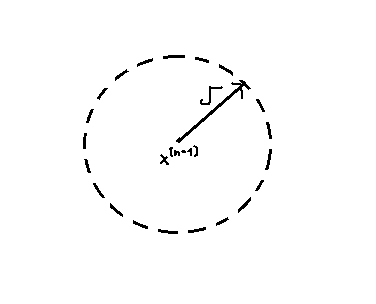
\includegraphics[scale=0.5]{krogla_3_4_1} \\
    (Povrnljivost - povsod, kjer neničelne verjetnosti, jemlje $\infty$-krat.) \\
    (To pomeni $q(y \mid x) = \frac{1}{Vol(K_{\delta}(x))} \cdot 1_{K_{\delta}(x)} (y)$ (namesto klasične uporabimo $\infty$ metriko).)
  \item $(Y \mid X^{(n-1)} = x^{(n-1)}) \sim N\left(x^{(n-1)}, \Sigma\right)$ za fiksno $\Sigma$. \\
    (To pomeni $q(y \mid x) = (2 \pi)^{-\frac{dim}{2}} (det \Sigma)^{-\frac{1}{2}} e^{-\frac{1}{2} \langle \Sigma^{-1}(y-x), (y-x)\rangle}$
      - simetričnost \checkmark.) \\
    V tem primeru je $Y|X^{(n-1)} = X^{(n-1)} + N(0, \Sigma)$.
\end{enumerate}
Metropolisov algoritem tipično nima ECLI :(.

\subsection{Metropolis-Hastingov algoritem}

Tu predlagane gostote $q(y \mid x)$ ne zadoščajo simetričnosti.
V algoritmu namesto $\rho$ iz 3.4.1. uporabimo
\begin{equation*}
  \rho = \rho\left(x^{(n-1)}, y\right) = \min \{1, \frac{f(y)}{f\left(x^{(n-1)}\right)} \cdot
    \frac{q\left(x^{(n-1)} \mid y\right)}{q\left(y \mid x^{(n-1)}\right)}\}
\end{equation*}
(in $\rho = 1$ če $f\left(x^{(n-1)}\right) \cdot q\left(y \mid x^{(n-1)}\right) = 0$). \\
\underline{Enake lastnosti kot prej:}
\begin{itemize}
  \item vedno dobimo verigo s stacionarno porazdelitvijo $f$
  \item če $\forall x: \; q(\_, x^{(n)})$ dopušča kandidate iz $\{f > 0\}$ (v končno korakih), velja EVZŠ (blagi pogoji).
\end{itemize}
Dobimo pa še: \\
- pri primernih predpostavkah na $q$ dobimo tudi ECLI.
\begin{exmp}[\sn{Neodvisni} Hastingov algoritem]
  Vedno \sn{funkcionira} (teoretično) $q(y \mid x) = q(y)$ za neko fiksno porazdelitev z gostoto $g$, kjer $g(y) > 0$ za $\forall f(y) > 0$.
\end{exmp}


% 8. predavanje: 6.11.

\subsection{Gibsov vzorčevalnik}

Gibsov vzorčevalnik je algoritem za konstrukcijo markovske verige s ciljno gostoto $f(x,y)$ (ali $f(x_1 \dots x_n)$)
na podlagi vzorčenja iz \sn{gostot} $f(x \mid y)$ ali $f(y \mid x)$. \\
\underline{Motivacija}: proučujemo vzorčni model z gostotami $f(x \mid \theta_1, \theta_2) = f(x \mid \theta)$,
ki je tak, da znamo simulirati neko vzorčenje iz $f(\theta_1 \mid \theta_2, x)$ in $f(\theta_2 \mid \theta_1, x)$,
ne pa (neposredno) iz $f(\theta_1, \theta_2 \mid x)$. \\
\underline{Opis algoritma}.
\begin{enumerate}[label=(\roman*)]
  \item Vzorčimo $y_0$ iz neke porazdelitve ali pa $y_0$ določimo. \\
    Vzorčimo $x_0$ iz pogojne porazdelitve $f(X \mid y_0)$.
  \item Če poznamo $(x_{n-1}, y_{n-1})$, vzorčimo najprej $y_n$ iz $f(x \mid x_{n-1})$,
    potem pa še $x_n$ iz $f(y \mid y_n)$ (temu koraku oz. njegovim podkorakom pravimo \sn{osveževanje}).
\end{enumerate}
Dobimo zaporedje s.s. (ali DN)
\begin{equation*}
  X^{(0)} = (x_0, y_0), \; X^{(1)} = (x_1, y_1), \; X^{(2)} = (x_2, y_2) \text{ itd.}
\end{equation*}
Izkaže se, da so zaporedja
\begin{align*}
  &X^{(0)}, X^{(1)}, X^{(2)} \dots \\
  &X_0, X_1, X_2 \dots \\
  &Y_0, Y_1, Y_2 \dots \\
\end{align*}
markovske verige in da ima veriga $\{X^{(i)} \mid n\}$ stacionarno porazdelitev $f(x,y)$.
Pri blagih pogojih je ta veriga ergodična.
\begin{exmp} \text{} \\
  Tipična aplikacija v Bayesovi statistiki je: \\
  privzemimo model $f(x \mid \theta_1, \theta_2)$ z apriorno gostoto $f(\theta_1, \theta_2) = f(\theta_1), f(\theta_2)$,
  kjer je $f(\theta_1)$ iz konjugirane družine k modelu $f(x \mid \theta_1, \text{KONST})$,
  $f(\theta_2)$ pa je iz konjugirane družine k modelu $f(x \mid \text{KONST}, \theta_2)$,
  iz katerih znamo simulirati NEP vzorčenje. \\
  Polna aposteriorna porazdelitev
  \begin{equation*}
    f(\theta_1, \theta_2 \mid x) = \frac{f(x \mid \theta_1, \theta_2) \cdot f(\theta_1) \cdot f(\theta_2)}{f(x)}
  \end{equation*}
  je tipično nedostopna, pač pa velja
  \begin{equation}
    \label{apost-theta1,2}
    f(\theta_1 \mid \theta_2, x) = \frac{f(x \mid \theta_1, \theta_2) \cdot f(\theta_1 \mid \theta_2)}{f(x \mid \theta_2)}
    = \frac{f(x \mid \theta_1, \theta_2) \cdot f(\theta_1)}{f(x \mid \theta_2)},
  \end{equation}
  kar je aposteriorna gostota Bayesovega modela z gostotami $f(x \mid \theta_1, \theta_2)$ iz apriorne gostote $f(\theta_1)$,
  kjer $\theta_2$ razumemo kot konstanto.
  Po našem premisleku je torej $f(\theta_1 \mid \theta_2, x)$ iz \sn{prave} konjugirane družine.
  Simetrično je
  \begin{equation*}
    f(\theta_2 \mid \theta_1, x) = \frac{f(x \mid \theta_1, \theta_2) \cdot f(\theta_2)}{f(x \mid \theta_1)}
  \end{equation*}
  iz \sn{znane} konjugirane družine. \\
  Konkretno si oglejmo enorazsežni NEP-normalni model
  \begin{equation}
    \label{NEP-normalni-model}
    (X \mid \mu, \sigma^2) \sim N\left(\begin{bmatrix}\mu \\ \vdots \\ \mu\end{bmatrix}, \sigma^2 I\right)
  \end{equation}
  z gostotami
  \begin{equation*}
    f(x_1 \dots x_n \mid \mu, \sigma^2) = f(x \mid \mu, \sigma^2) =
    \left(2 \pi \sigma^2\right)^{-\frac{n}{2}} e^{-\frac{1}{2 \sigma^2} \cdot \sum_{i=1}^{n} (x_i-\mu)^2}.
  \end{equation*}
  Vemo, da je $\{N(\mu_{*}, \tau_{*}^2) \mid \mu_{*} \in \R, \tau_{*}^2 \in (0, \infty)\}$
  konjugirana k enoparametričnim modelom z gostotami \refeq{NEP-normalni-model}, kjer $\sigma^2$ poznamo. \\
  Izkaže se (vaja), da je družina $\{\text{InvGama}(a,b) \mid a,b \in (0, \infty)\}$
  konjugirana k enoparametričnim modelom z gostotami \refeq{NEP-normalni-model}, kjer $\mu$ poznamo.
  Tu je $Y \sim \text{InvGama}(a,b) \iff \frac{1}{Y} \sim \text{Gama}(a,b)$, velja
  \begin{equation*}
    f_{\text{InvGama}(a,b)}(y) = \frac{b^a}{\Gamma(a)} y^{-a-1} e^{-\frac{b}{y}}.
  \end{equation*}
  Vemo: pri $f(\mu) = f_{N(\mu_{*}, \tau_{*}^2)}(\mu)$ je
  \begin{equation*}
    f(\mu \mid \sigma^2, x) \stackrel{\refeq{apost-theta1,2}}{=}
      f_{N\left(\frac{\frac{\sigma^2}{n}}{\frac{\sigma^2}{n} + \tau_{*}^2} \mu_{*} + 
                \frac{\tau_{*}^2}{\frac{\sigma^2}{n} + \tau_{*}^2} \overline{x},
                \frac{\frac{\sigma^2}{n} \cdot \tau_{*}^2}{\frac{\sigma^2}{n} + \tau_{*}^2}\right)}(\mu).
  \end{equation*}
  Vidimo: pri $f(\sigma^2) = f_{\text{InvGama}(a,b)}(\sigma^2)$ je
  \begin{equation*}
    f(\sigma^2 \mid \mu, x) =
      f_{\text{InvGama}\left(a+\frac{n}{2}, b+\frac{1}{2}\sum_{i=1}^{n}(x_i-\mu)^2\right)}(\sigma^2).
  \end{equation*}
  \underline{Gibsov vzorčevalnik}: ciljna porazdelitev $f(\mu, \sigma^2 \mid x)$.
  \begin{enumerate}[label=(\roman*)]
    \item Določimo $\sigma_0^2 = 1$. Vzorčimo $\mu_0$ iz
      \begin{equation*}
        f_{N\left(\frac{\frac{1}{n}}{\frac{1}{n} + \tau_{*}^2} \mu +
                  \frac{\tau_{*}^2}{\frac{1}{n} + \tau_{*}^2} \overline{x},
                  \frac{\frac{1}{n} \tau_{*}^2}{\frac{1}{n} + \tau_{*}^2}\right)},
      \end{equation*}
    \item vzorčimo $\sigma_1^2$ iz $f(\sigma^2 \mid \mu_0, x)$, \\
      vzorčimo $\mu_1^2$ iz $\dots$ \\
      $\vdots$
  \end{enumerate}
  (Blagi pogoji so izpolnjeni, veriga ergodična.)
\end{exmp}


% 10. predavanje: 14.11.

\section{Markovske verige z zveznim prostorom stanj - appendix}

Markovska veriga \sn{na} $\Sigma$ v diskretnem času je zaporedje merljivih preslikav $X_i: \Omega \to \Sigma$
$(i = 0, 1, 2 \dots)$, kjer je $\Omega$ verjetnostni prostor, $\Sigma$ merljiv prostor in velja
\begin{equation}
  P(X_n \in A \mid X_{n-1} = x_{n-1} \dots X_0 = x_0) = P(X_n \in A \mid X_{n-1} = x_{n-1})
  \label{markovska-lastnost-A}
\end{equation}
za vse $n \in \N, A \subset \Sigma$ in vse n-terice $x_0 \dots x_{n-1} \in \Sigma$. \\
Tu je $\{P(\_ \mid x) \mid x \in \Sigma\}$ družina verjetnostnih mer na $\Sigma$, za katero velja,
da je za vsako merljivo množico $A \subset \Sigma$ preslikava $\Sigma \to [0,1]$, $x \mapsto \P(A \mid x)$ merljiva. \\
Prostoru $\Sigma$ pravimo parameter stanj, $X_i$ so členi verige,
lastnosti \refeq{markovska-lastnost-A} pa pravimo markovska lastnost. \\
Tu se bomo omejili na Borelove množice $\Sigma \subset \R^r$ (z Borelovo $\sigma$-algebro.) \\
Poudarimo, da so verjetnosti $P(_ \mid x)$ (pravimo jim \sn{prehodne verjetnosti}) neodvisne od $n$
(torej za vse $n$ enake).
\begin{exmp} \text{} \\
  Če ima $X_0$ neko porazdelitev in velja $X_n = X_{n-1} + \varepsilon_n$
  (kjer so $X_0, \varepsilon_1 \dots$ neodvisne in $\epsilon_0 \sim N(0, V)$ za $V \in \P(r)$ (V je s.p.d.))
  in $X_0, X_1, X_2 \dots$ markovska veriga in velja
  \begin{equation*}
    P(A \mid x) = P(N(x, V) \in A).
  \end{equation*}
\end{exmp}
\begin{exmp}
  Metropolis-Hastingovova veriga:
  \begin{enumerate}[label=(\arabic*)]
    \item imamo $X_0 = x_0$,
    \item če je $X_{n-1} = x$, potem realizacijo od $X_n$ dobimo takole:
      \begin{enumerate}[label=(\roman*)]
        \item vzorčimo $y$ iz predlagane porazdelitve $dP_{(Y \mid x)} = q(y \mid x) d\nu(y)$
        \item vzorčimo $u = U \sim U(0,1)$ in sprejmemo $X_n = y$, če $u \leq \rho(x, y)$
          oz. $X_n = x$, če $u > \rho(x,y)$, kjer
          \begin{equation*}
            \rho(x,y) = \begin{cases}
              \min \{1, \frac{f(y)}{f(x)} \cdot \frac{q(x \mid y)}{q(y \mid x)}\}; f(x) q(y \mid x) \neq 0 \\
              1; f(x) q(y \mid x) = 0
            \end{cases}
          \end{equation*}
          Tu je $f$ ciljna gostota (glede na $\nu$),
      \end{enumerate}
    \item 
      \begin{align*}
        &P(X_n \in A \mid X_{n-1}=x) \\
        &= \int_{y \in \Sigma} P(X_n \in A \mid Y=y, X_{n-1}=x) dP_{(Y \mid x)}(x) \\
        &= \int_{y \in \Sigma} \int_{u=0}^{1} P(X_n \in A \mid U=u, Y=y, X_{n-1}=x)
          \cdot dP_{(U \mid Y=y, X_{n-1}=x)}(u) d\nu(y) \\
        &= \int_{y \in \Sigma}
          \left(\int_{u=0}^{\rho(x,y)} \dots du + \int_{u=\rho(x,y)}^{1} \dots du\right)
          q(y \mid x) d\nu(y) \\
        &= \int_{y \in \Sigma} \left(1_A(y) \cdot q(y \mid x) + 1_A(x) \cdot (1-\rho(x,y))\right)
          q(y \mid x) d\nu(y) \\
        &= \int_{y \in A} \rho(x, y) q(y \mid x) d\nu(y)
          + 1_A(x) \int_{y \in \Sigma} (1-\rho(x,y)) q(y \mid x) d\nu(y).
      \end{align*}
      Privzemimo, da $\nu$ nima atomov: $\nu({x}) = 0$ za vsak $x$:
      \begin{equation*}
        \implies P(X_n \in A \mid X_{n-1} = x) = \int_{y \in \Sigma} (1-\rho(x,y)) q(y \mid x) d\nu(y).
      \end{equation*}
      To je tipično $u$ pozitivna verjetnost.
      To pomeni, da imajo prehodne verjetnosti atome $u$: $P({x} \mid x) > 0$ (vsaj za nekatere $x$).
  \end{enumerate}
\end{exmp}
\begin{defn} \text{} \\
  Porazdelitev $\pi$ je stacionarna za verigo $\{X_i\}$, če iz $X_{n-1} \sim \pi$ sledi $X_n \sim \pi$.
\end{defn}
\begin{claim} \text{} \\
  Porazdelitev $f d\nu$ je stacionarna porazdelitev M-H verige.
\end{claim}
\begin{pro} \text{} \\
  Privzemimo $dP_{X_{n-1}} = f d\nu$ in računajmo
  \begin{align*}
    P(X_n \in A) =& \int_{x \in \Sigma} P(X_n \in A \mid X_{n-1} = x) dP_{X_{n-1}}(x) \\
    =& \int_{x \in \Sigma} \int_{y \in A} \rho(x,y) q(y \mid x) f(y) d\nu(y) d\nu(x) \\
      &+ \int_{x \in A} \int_{y \in \Sigma} q(x \mid y) d\nu(y) f(x) d\nu(x) \\
      &- \int_{x \in A} \int_{y \in \Sigma} \rho(x, y) q(x \mid y) f(x) d\nu(y) d\nu(x).
  \end{align*}
  Upoštevamo
  \begin{equation*}
    \int_{y \in \Sigma} q(x \mid y) f(x) d\nu(y) = 1.
  \end{equation*}
  Spomnimo se:
  \begin{equation*}
    \rho(x,y) = \begin{cases}
      \min \{1, \frac{f(y)}{f(x)} \cdot \frac{q(x \mid y)}{q(y \mid x)}\}; f(x) q(y \mid x) \neq 0 \\
      1; f(x) q(y \mid x) = 0
    \end{cases}
  \end{equation*}
  Vidimo, da velja enakost (za $\forall x, y$)
  \begin{equation*}
    \rho(x,y) q(y \mid x) f(x) = \rho(y,x) q(x \mid y) f(y)
  \end{equation*}
  in
  \begin{equation*}
    \int_{x \in \Sigma} \int_{y \in A} \rho(x,y) q(y \mid x) f(y) d\nu(y) d\nu(x) =
    \int_{y \in \Sigma} \int_{x \in A} \rho(y,x) q(x \mid y) f(x) d\nu(x) d\nu(y).
  \end{equation*}
  Zato je
  \begin{equation*}
    P(X_n \in A) = \int_{x \in A} f(x) d\nu(y).
  \end{equation*}
\end{pro}
Prehodne verjetnosti $P(_ \mid x)$ generirajo verigo prehodnih verjetnosti \\
$P(A \mid x) = P(X_n \in A \mid X_0 = x)$. \\
To verjetnost, da veriga obišče $A$ v času $n$ ob pogoju, da je začela v $x$,
želeni lastnosti (ki implicirata ustrezna ERVŠ) sta
\begin{itemize}
  \item $||P^n(_ \mid x) - \pi|| \stackrel{n \to \infty}{\to} 0$ za skoraj vse $x$,
  \item $||P^n(_ \mid x) - \pi|| \stackrel{n \to \infty}{\to} 0$ enakomerno v $x$,
\end{itemize}
kjer za predznačeno mero $\mu$ definiramo normo totalne variacije
\begin{equation*}
  || u || = \sup_A |\mu(A)|.
\end{equation*}
Za osnovne lastnosti $P^n(A \mid x)$ izračunajmo
\begin{align*}
  &P(X_n \in A_n, X_{n-1} \in A_{n-1} \dots X_1 \in A_1 \mid X_0=x_0) \\
  &=\int_{x_1 \in \sigma} P(X_n \in A_n \dots X_1 \in A_1 \mid X_1=x_1, X_0=x_0) dP_{(X_1 \mid X_0=x_0)}(x_1) \\
  &=\int_{x_1 \in A_1} P(X_n \in A_n \dots X_2 \in A_2 \mid X_1=x_1, X_0=x_0) dP_{(X_1 \mid X_0=x_0)}(x_1 \mid x_0) \\
  &=\int_{x_1 \in A_1} \int_{x_2 \in \Sigma}
    P(X_n \in A_n \dots X_2 \in A_2 \mid X_2=x_2, X_1=x_1, X_0=x_0) dP(x_2 \mid x_1) dP(x_1 \mid x_0) \\
  &= \dots \\
  &= \int_{x_1 \in A_1} \dots \int_{x_n \in A_n} dP(x_n \mid x_{n-1}) \dots dP(x_1 \mid x_0).
\end{align*}
\underline{Posebej}:
\begin{equation*}
  P^n(A \mid x) = \int_{x_1 \in \Sigma} \dots \int_{x_{n-1} \in \Sigma} \int_{x_n \in A}
    dP(x_n \mid x_{n-1}) \dots dP(x_1 \mid x).
\end{equation*}
Od tod sledi
\begin{align*}
  P^n(A \mid x) &= \int_{x_1 \in \Sigma} \dots \int_{x_m \in \Sigma}
    \left(\int_{x_{m+1} \in \Sigma} \dots \int_{x_n \in A} dP(x_n \mid x_{n-1} \dots dP(x_{m+1} \mid x_m))\right) \\
  &\cdot dP(x_m \mid x_{m-1}) \dots dP(x_1 \mid x_0).
\end{align*}
Tukaj je
\begin{equation*}
  \int_{x_{m+1} \in \Sigma} \dots \int_{x_n \in A} dP(x_n \mid x_{n-1} \dots dP(x_{m+1} \mid x_m)) = P^{n-m}(A \mid x_m)
\end{equation*}
in zato
\begin{equation*}
  P^n(A \mid x) = \int_{x_1 \in \Sigma} P^{n-m} (A \mid x_m) \cdot dP^m(x_m \mid x).
\end{equation*}
Tej enakosti rečemo enakost Chapman-Kolmogorova.


% 9. predavanje: 13.11.

\chapter{Normalni modeli}


\underline{Uvodni zgled}: 1-razsežni \sn{NEP-normalni} model, kjer je
$(X \mid \mu, \sigma^2) \sim N(\left(\begin{bmatrix}\mu & \vdots & \mu\end{bmatrix}, \sigma^2 I_{n \times n}\right))$
z vzorčnimi gostotami
\begin{equation}
  f(x \mid \mu, \sigma^2) = \left(2 \pi \sigma^2\right)^{-\frac{n}{2}} e^{-\frac{1}{2 \sigma^2} \left(\sum_{i=1}^{n} (x_i-\mu)^2\right)}.
  \label{normalni-gostota-x}
\end{equation}
Izkaže se, da je konjugirana družina apriornih gostot podana kot
\begin{equation}
  f(\mu, \sigma^2) = f_{\text{InvGama}(a,b)}(\sigma^2) \cdot f_{N\left(\mu_0, \frac{\sigma^2}{\kappa_0}\right)}(\mu).
  \label{normalni-apriorna}
\end{equation}
(Za vajo lahko izpeljete; razcepite $\psi = \psi_1 + \psi_2$ ($\log$ ?) $\to$ $\tau_1, \tau_2$ namesto $\tau$). \\
Tu so $\mu_0 \in \R, a, b, \kappa_0 \in (0, \infty)$ parametri konjugirane družine;
$\kappa_0$ interpretiramo kot število prostorskih stopenj (fiktivno).


\section{Dvofazna predstavitev}

Privzemimo razcep $\vartheta = (\vartheta_1, \vartheta_2)$ in zapišimo
\begin{equation*}
  f(\vartheta_1, \vartheta_2) = f(\vartheta_1 \mid \vartheta_2) \cdot f(\vartheta_2).
\end{equation*}
Za aposteriorno gostoto pri $X = x$ velja
\begin{equation*}
  f(\vartheta_1, \vartheta_2 \mid x) = \frac{f(x \mid \vartheta_1, \vartheta_2) \cdot f(\vartheta_1 \mid \vartheta_2)}{f(x \mid \vartheta_2)}
    \cdot \frac{f(x \mid \vartheta_2) \cdot f(\vartheta_2)}{f(x)}
\end{equation*}
oz.
\begin{equation*}
  f(\vartheta_1, \vartheta_2 \mid x) = f(\vartheta_1 \mid \vartheta_2, x) \cdot f(\vartheta_2 \mid x).
\end{equation*}
Tu je $f(\vartheta_1 \mid \vartheta_2, x)$ aposteriorna gostota modela z vzorčnimi gostotami $f(x \mid \vartheta_2)$
in apriorno gostoto $f(\vartheta_2$). \\
Tipično je $f(\vartheta_1 \mid \vartheta_2, x)$ enostavneje izračunati (eksplicitno) kot $f(\vartheta_2 \mid x)$,
ker za slednje potrebujemo še $f(x \mid \vartheta_2)$. \\
Načeloma lahko $f(x \mid \vartheta_2)$ izračunamo z integriranjem:
\begin{equation*}
  f(x \mid \vartheta_2) = \int f(x \mid \vartheta_1, \vartheta_2) \cdot f(\vartheta_1 \mid \vartheta_2) d\vartheta_1,
\end{equation*}
vendar :( \\
\underline{Aplicirajmo} na vzorčne gostote z \refeq{normalni-gostota-x} z apriorno \refeq{normalni-apriorna}.
\begin{enumerate}[label=(\roman*)]
  \item $f(\mu \mid \sigma^2, x)$ \sn{pripada} modelu $(X \mid \mu) \sim
    N\left(\begin{bmatrix}\mu\\\vdots\\\mu\end{bmatrix}, \sigma^2 I\right)$ ($\sigma^2$ konst.) za apriorno
    $M \sim N\left(\mu_0, \frac{\sigma^2}{\kappa_0}\right) = N(\mu_0, \tau_0^2)$. \\
    To pomeni $f(\mu \mid \sigma^2, x) \leftrightarrow N(\mu, \tau_0^2)$, kjer je
    \begin{equation*}
      \mu_1 = \frac{\frac{\sigma^2}{n}}{\frac{\sigma^2}{n} + \tau_0^2} \mu_0 + \frac{\tau_0^2}{\frac{\sigma^2}{n} + \tau_0^2} \overline{x}
    \end{equation*}
    in
    \begin{equation*}
      \tau_1^2 = \frac{\frac{\sigma^2}{n} \cdot \tau_0^2}{\frac{\sigma^2}{n} + \tau_0^2} = \frac{\sigma^2}{n + \kappa_0}.
    \end{equation*}
    Interpretacija variance: več primerov.
  \item Za $f(\sigma^2 \mid x)$ potrebujemo $f(x \mid \sigma^2)$. \\
    DN: intergirajte. \\
    Oglejmo si raje
    \begin{align*}
      f(x, \mu \mid \sigma^2) &= f(x \mid \mu, \sigma^2) \cdot f(\mu \mid \sigma^2) \\
      &\propto e^{-\frac{1}{2\sigma^2} \sum_{i=1}^{n} (x_i - \mu)^2} \cdot
        e^{-\frac{1}{2 \left(\frac{\sigma^2}{\kappa_0}\right)} (\mu - \mu_0)^2} \\
      &= e^{-\frac{1}{2} \left\langle W \begin{bmatrix}x_1\\\vdots\\x_n\\\mu\end{bmatrix},
        \begin{bmatrix}x_1\\\vdots\\x_n\\\mu\end{bmatrix} \right\rangle},
    \end{align*}
    kjer je
    \begin{equation*}
      W = \begin{bmatrix}
        \frac{1}{\sigma^2} & \dots & 0 & -\frac{1}{\sigma^2} \\
        0 & \dots & \vdots & -\frac{1}{\sigma^2} \\
        \vdots & \vdots & \frac{1}{\sigma^2} & -\frac{1}{\sigma^2} \\
        -\frac{1}{\sigma^2} & \frac{1}{\sigma^2} & \dots & \frac{\kappa_0 + n}{\sigma^2}
      \end{bmatrix}.
    \end{equation*}
    Vidimo, da je $(X, M \mid V \sim \sigma^2)$ normalna porazdelitev $\implies \; (X \mid V \sim \sigma^2)$ je kot robna tudi normalna. \\
    $\stackrel{!!}{\implies}$ potrebujemo le $E(X \mid V \sim \sigma^2)$ in $Var(X \mid V \sim \sigma^2)$. \\
    Vemo:
    \begin{align*}
      E(X \mid V \sim \sigma^2) =& E(E(X \mid M, V) \mid V \sim \sigma^2) \text{ in} \\
      Var(X \mid V \sim \sigma^2) =& E(Var(X \mid M, V) \mid V \sim \sigma^2) + \\
      &Var(E(X \mid M, V) \mid V \sim \sigma^2).
    \end{align*}
    Naprej:
    \begin{align*}
      &E(X \mid M = \mu, V \sim \sigma^2) = \mu \cdot \begin{bmatrix}1\\\vdots\\1\end{bmatrix}
        \implies E(X \mid M, V) = \begin{bmatrix}1\\\vdots\\1\end{bmatrix} \cdot M \\
      &Var(X \mid M = \mu, V \sim \sigma^2) = \sigma^2 I \implies Var(X \mid M, V) = V \cdot I.
    \end{align*}
    Sledi:
    \begin{align*}
      &E(X \mid V \sim \sigma^2) = E\left(\begin{bmatrix}1\\\vdots\\1\end{bmatrix} M \mid V \sim \sigma\right) =
        \begin{bmatrix}1\\\vdots\\1\end{bmatrix} \mu_0 \text{ in} \\
      &Var(X \mid V \sim \sigma^2) = \sigma^2 I +
        \begin{bmatrix}1\\\vdots\\1\end{bmatrix} Var(M \mid V \sim \sigma^2) \begin{bmatrix}1&\cdots&1\end{bmatrix} \\
      &= \sigma^2 \left(I + \frac{1}{\kappa_0} \begin{bmatrix}1&\dots&1\\\vdots&&\vdots\\1&\dots&1\end{bmatrix}\right).
    \end{align*}
    Lahko zapišemo
    \begin{align*}
      f(x \mid \sigma^2) &= (2 \pi \sigma^2)^{-\frac{n}{2}} \cdot
        det \left(I + \frac{1}{\kappa_0} \begin{bmatrix}1&\dots&1\\\vdots&&\vdots\\1&\dots&1\end{bmatrix}\right)^{-1} \\
      &\cdot e^{-\frac{1}{2\sigma^2} \left\langle 
          \left(I + \frac{1}{\kappa_0} \begin{bmatrix}1&\dots&1\\\vdots&&\vdots\\1&\dots&1\end{bmatrix}\right)^{-1}
          \left(x - \begin{bmatrix}\mu_0\\\vdots\\\mu_0\end{bmatrix}\right), x - \begin{bmatrix}\mu_0\\\vdots\\\mu_0\\\mu_0\end{bmatrix}
        \right\rangle}.
    \end{align*}
    Velja še
    \begin{align*}
      &f(\sigma^2) = f_{\text{InvGama}}(\sigma^2) = \frac{b^a}{\gamma(a)} \cdot (\sigma^2)^{-a-1} \cdot e^{-\frac{b}{\sigma^2}} \\
      \implies &f(\sigma^2 \mid x) \propto (\sigma^2)^{-\frac{n}{2}} \cdot
        e^{-\frac{1}{\sigma^2} \frac{1}{2} \left(\langle \dots, \dots \rangle\right)} \cdot (\sigma^2)^{-a-1} e^{-\frac{b}{\sigma^2}} \\
        &\leftrightarrow \text{InvGama}\left(a + \frac{n}{2},
          b + \frac{1}{2} \left\langle
            \left(I + \frac{1}{\kappa_0} \begin{bmatrix}1&\dots&1\\\vdots&&\vdots\\1&\dots&1\end{bmatrix}\right)^{-1}
            \left(x - \begin{bmatrix}\mu_0\\\vdots\\\mu_0\end{bmatrix}\right), x - \begin{bmatrix}\mu_0\\\vdots\\\mu_0\end{bmatrix}
          \right\rangle\right)
    \end{align*}
    $\leftrightarrow$: konjugirana porazdelitev. \\
    Prepričali smo se, da je opisana družina apriornih porazdelitev konjugirana, in sicer
    \begin{itemize}
      \item $a \to a + \frac{n}{2}$
      \item $b \to b + \frac{1}{2} \langle \dots, \dots \rangle$
      \item $\mu_0 \to \frac{\kappa_0}{\kappa_0 + n} \mu_0 + \frac{n}{\kappa_0 + n} \overline{x}$
      \item $\kappa_0 \to \kappa_0 + n$.
    \end{itemize}
    Nova $b$ in $\mu_0$ sta odvisna od realizacije $(x_1 \dots x_n)$. \\
    $b + \frac{1}{2} \left(\sum_{i=1}^{n} (x_i - \overline{x})^2 + \frac{n \cdot \kappa_0}{\kappa_0 + n} (\overline{x} - \mu_0)^2\right)$
\end{enumerate}


\section{Hierarhični modeli}

Spomnimo se na normalni model \sn{preizkušnja $m$ terapij}.
Frekvencistično gledamo neodvisne skupine s.s. \\
\begin{tabular}{c @{\hspace{2\tabcolsep}} *{4}{c}}
  $X_{1,1}$ & $X_{1,2}$ & $\dots$ & $X_{1,m}$ \\
  $\vdots$ & $\vdots$ & & $X_{n_m, m}$ \\
  $X_{n_1, 1}$ & $\vdots$ & & \\
  & $X_{n_2, 2}$ & &
\end{tabular}. \\
Velikosti $n_1 + \dots + n_m = n$. \\
Funkcija neodvisnosti: $X_{ij} \sim N(\mu_j, \sigma^2)$. \\
Vse variance so enaka (homoskelastičnost) zaradi \sn{preprostosti}. \\
Najbolj nas zanimajo (ocene) za $\mu_j$ in $\sigma^2$, \sn{optimalne} frekventistične cenilke so:
\begin{align*}
  &\hat{\mu_j} = \frac{1}{n_j} \sum_{i=1}^{n_j} X_{ij} = \overline{X_{.j}} \\
  &\hat{\sigma} = \frac{1}{n-m} \sum_{j=1}^m \sum_{i=1}^{n_j} (X_{ij} - \overline{X_{.j}})^2.
\end{align*}


% 11. predavanje: 20.11.

\underline{Zadnjič}: model $m$ terapij $N(\mu_j, \sigma^2) \; (1 \leq j \leq m)$. \\
Po preizkušnju domnev je glavna t.i. domneva homogenosti \\
$\mu_1 = \mu_2 = \dots = \mu_m$. \\
V pridruženem Bayesovem modelu začnemo z idejo, da so $\mu_j$ \sn{poustvarjanje} nekega \sn{izhodiščnega} $\mu_0$. \\
$\sigma^2$ našega homoskelastičnega modela je znana. \\
$\mu_0, \tau_0^2, a, b$ \\
$\downarrow$ \\
$\mu, \eta^2 \in N(\mu_0, \tau_0^2) \times \text{InvGama}(a,b)$ - Bayesov parameter \\
$\downarrow$ \\
$\mu_1 \dots \mu_m \in N(\mu, \eta^2) \times \dots \times N(\mu, \eta^2)$ - $\phi$ - Bayesov parameter \\
$\downarrow$ (neodvisno) \\
$x_{i_1} \in N(\mu_1, \sigma^2) \; (1 \leq i \leq n_1) \dots x_{i_m} \in N(\mu_m, \sigma^2) \; (1 \leq i \leq n_m)$
- $\vartheta$ - vzorec \\
(večji $\tau^2$, bolj $\mu_i$ različni). \\

\subsection{Abstraktna opredelitev hierarhičnega modela}

Bayesov parameter je oblike $(\vartheta, \phi)$ kjer $\phi$ imenujemo hiperparameter,
$\vartheta$ pa populacijski parameter.
Za vzorčne gostote velja temeljni privzetek \\
(HM - hierarhični model) $f(x \mid \vartheta, \phi) = f(x \mid \vartheta)$. \\
Aposteriorne gostote bi lahko predstavili kot
\begin{align*}
  f(\vartheta \mid \phi, x) &= \frac{f(x \mid \vartheta, \phi) f(\vartheta \mid \phi) f(\phi)}{f(x)} \\
  &= \frac{f(x \mid \vartheta) f(\vartheta)}{f(x)} \cdot \frac{f(\vartheta \mid \phi) f(\phi)}{f(\vartheta)} \\
  &= f(\vartheta \mid x) f(\phi \mid \vartheta).
\end{align*}
Ta predstavitev tipično ni uporabna, ker ne poznamo $f(\vartheta)$. Zato raje
\begin{itemize}
  \item $f(\vartheta \mid \phi, x) = \frac{f(x \mid \vartheta, \phi) f(\vartheta \mid \phi)}{f(x \mid \phi)}$:
    aposteriorna gostota modela z vzorčnimi $f(x \mid \vartheta)$ in apriornimi $f(\vartheta \mid \phi)$,
  \item $f(\phi \mid \vartheta, x) = \frac{f(x \mid \vartheta) f(\phi \mid \vartheta)}{f(x \mid \vartheta)}$:
    aposteriorna gostota modela z vzorčnimi $f(\vartheta \mid \phi)$ in apriornimi $f(\phi)$
\end{itemize}
($\implies$ z Gibsom $f(\vartheta, \phi \mid x)$). \\
Aplicirajmo na naš zgled: \\
$\phi = (\mu, \eta^2)$ \\
$n = \sum_{j=1}^{m} n_j$ \\
$\vartheta = (\mu_1 \dots \mu_m)$ \\
\begin{align*}
  f([x_{ij}] \mid \mu_1 \dots \mu_m) &= \prod_{j=1}^{m} \left(2 \pi \sigma^2\right)^{-\frac{n}{2}}
    e^{-\frac{1}{2 \sigma^2} \sum_{i=1}^{n_j} (x_{ij} - \mu_j)^2} \\
  &= \left(2 \pi \sigma^2\right)^{-\frac{n}{2}}
    e^{-\frac{1}{2 \sigma^2} \sum_{j=1}^{m} \sum_{i=1}^{n_j} (x_{ij} - \mu_j)^2}
\end{align*}
$j = 1 \dots m, \; i = 1 \dots n_j$. \\
Populacijska apriorna:
\begin{equation*}
  f(\mu_1 \dots \mu_m \mid \mu, \eta^2) = \left(2 \pi \eta^2\right)^{-\frac{n}{2}}
    e^{-\frac{1}{2 \eta^2} \sum_{j=1}^{m} (\mu_j - \mu)^2},
\end{equation*}
hiperapriorna:
\begin{equation*}
  f(\mu, \sigma^2) = f_{N(\mu_0, \tau_0^2)}(\mu) \cdot f_{\text{InvGama}(a,b)} (\eta^2).
\end{equation*}
\begin{align*}
  &f(\mu_1 \dots \mu_m \mid \mu, \eta^2, [x_{ij}]) \\
  &\propto \prod_{i=1}^{m} e^{-\frac{1}{2 \sigma^2} \sum_{i=1}^{n_j} (x_{ij} - \mu_j)^2}
   \cdot e^{-\frac{1}{2 \eta^2} (\mu_j - \mu)^2}.
\end{align*}
Analogije z aposteriornim NEP-normalnim modelom:
\begin{itemize}
  \item $\sigma^2 - \sigma^2$
  \item $x_{ij} - x_i$
  \item $\mu_j - \mu$
  \item $\eta^2 - \tau_0^2$
  \item $\mu_j - \mu$
  \item $\mu - \mu_0$.
\end{itemize}
Ta pogojna aposteriorna porazdelitev je
\begin{equation*}
  \prod_{j=1}^{m} N \left( \frac{\frac{\sigma^2}{n_j}}{\frac{\sigma^2}{n_j} + \eta^2} \mu
    + \frac{\eta^2}{\frac{\sigma^2}{n_j} + \eta^2} \overline{x_{.j}},
    \frac{\frac{\sigma^2}{n_j} \cdot \eta^2}{\frac{\sigma^2}{n_j} + \eta^2} \right).
\end{equation*}
$f(\mu, \eta^2 \mid \mu_1 \dots \mu_m)$ 1-razsežni NEP-normalni model s polkonjugirano apriorno porazdelitvijo
\begin{align*}
  &f(\mu \mid \eta^2, \mu_1 \dots \mu_m) \dots
    N \left( \frac{\frac{\tau_0^2}{m}}{\frac{\tau_0^2}{m} + \tau_0^2} \mu_0
    + \frac{\tau_0^2}{\frac{\tau_0^2}{m} + \tau_0^2} \overline{\mu},
    \frac{\frac{\tau_0^2}{m} \cdot \tau_0^2}{\frac{\tau_0^2}{m} + \tau_0^2} \right) \\
  &f(\tau^2 \mid \mu, \mu_1 \dots \mu_m) \dots
    \text{InvGama}\left(a+\frac{m}{2}, b+\frac{1}{2}\sum_{i=1}^{m}(\mu_j-\mu)^2\right).
\end{align*}


% 12. predavanje: 21.11.

\begin{defn}
  Naj bo $\nu$ mera na $B(\Sigma)$.
  Tedaj je veriga $\{X_n\}$ \\
  $\nu$-ireducibilna, če iz $\nu(A) > 0$ sledi
  \begin{equation*}
    \forall x \; \exists m = n_n: \; P^n(A \mid x) = P(X_m \in A \mid X_0 = x) > 0.
  \end{equation*}
\end{defn}
Če naj velja EZVŠ, moramo vsako množico $A$, za katero
\begin{equation*}
  \pi(A) = \int_A d\pi(y) = \int_A f(y) dy > 0
\end{equation*}
obiskati neskončno-mnogokrat.
Torej nas v našem kontekstu zanima \\
$\pi$-ireducibilnost, kjer je $\pi$ stacionarna porazdelitev.
\begin{ex}
  Če iz $f(y) > 0$ sledi $q(y \mid x) > 0$, je M-H (Metropolis-Hastingova) veriga $\pi$-ireducibilna.
\end{ex}
\underline{Komentar}: zgornji pogoj je za praktične namene pogosto pomešan? (neuporaben?).
\begin{defn}
  Naj bo $\pi$ stacionarna porazdelitev verige $\{X_n\}$, ki je \\
  $\pi$-ireducibilna.
  Veriga $\{X_n\}$ je periodična s periodo $d \geq 2$, če obstajajo paroma disjunktne Borelove množice $E_0 \dots E_{d-1}$,
  za katere velja
  \begin{equation*}
    \forall i \in \{0 \dots d-1\} \; \forall x \in E_i: \; P({E_{i+1 \text{ mod } d}} \mid x) = 1.
  \end{equation*}
  Pripomnimo, da tedaj sledi
  \begin{equation*}
    \forall x \in E_i: \; P^d(E_i \mid x) = 1.
  \end{equation*}
\end{defn}
(Naj bo $x \in E_i$.
Tedaj
\begin{align*}
  P^2(E_{i+2 \text{ mod } d} \mid x) &= \int_{\Sigma} P(E_{i+2 \text{ mod } d} \mid y) dP(y \mid x) \\
  &\geq \int_{y \in E_{i+1 \text{ mod }    d}} \dots \\
  &= \int_{y \in E_{i+1 \text{ mod } d}} dP(y \mid x) = 1.)
\end{align*}
Če veriga ni periodična, je aperiodična.
\begin{claim}
  Če sta $f(y)$ in $q(y \mid x)$ pozitivni in zvezni povsod na $\Sigma = \R^r$ oz $\Sigma \times \Sigma = \R^r \times \R^r$,
  je $\pi$-ireducibilna M-H veriga tudi aperiodična.
\end{claim}
\begin{theorem}
  Če je M-H veriga $\pi$-ireducibilna in aperiodična, velja
  \begin{equation*}
    \lim_{n \to \infty} \sup_{A \in B\left(\R^r\right)} \left|P^n(A \mid x) - \pi(A)\right| = 0
  \end{equation*}
  $\pi = s.s. [x]$ (za s.g. vsak $x$).
\end{theorem}
\begin{theorem}
  Privzemimo $q(y \mid x) = q(y)$ za $\forall x$ (neodvisni M-H) in $q(y) > 0$ ter $f(y) > 0$.
  Če obstaja konstanta $M$, za katero je $\forall y: \; f(y) < M q(y)$, je M-H veriga ENAKOMERNO ERGODIČNA,
  obstaja zaporedje $r(n) \stackrel{n \to \infty}{\to} 0$, za katero velja $\sup_A \left|P^n(A \mid x) - \pi(A)\right| \leq r(n)$.
  Tu obstaja eksplicitni izraz za $r(n)$.
\end{theorem}
\begin{rem}
  Pri predpostavkah izreka zmano s A/R simulirati NEODVISNO vzorčenje iz $\pi$.
\end{rem}
\begin{defn}
  Naj bo $\pi$ stacionarna oprazdelitev verige $\{X_n\}$, ki je $\pi$-ireducibilna.
  Tedaj je ta veriga POVRNLJIVA, če iz $\pi(A) > 0$ sledi
  \begin{enumerate}[label=(\roman*)]
    \item $P(X_n \in A \text{ neskončno mnogokrat } \mid x) > 0$ za $\forall x$,
    \item $P(X_n \in A \text{ neskončno mnogokrat } \mid x) = 1$ za $\pi$-skoraj vse $x$.
  \end{enumerate}
\end{defn}
\begin{defn}
  Veriga je Harrisov povrnljiva, če velja (ii) za $\forall x$.
\end{defn}
\begin{theorem}
  Naj bo $\pi$ stacionarna porazdelitev verige $\{X_n\}$, ki je $\pi$-ireducibilna.
  Tedaj je veriga povrnljiva.
  \begin{itemize}
    \item Če je veriga še aperiodična, velja $\lim_{n \to \infty} \sup_A \left|P^n(A \mid x) - \pi(A)\right| = 0$ za vsak $x$
      ($\pi$-s.g. $[x]$).
    \item Če je veriga Harrisov povrnljiva,
      velja $\lim_{n \to \infty} \sup_A B\left(P^n(A \mid x) - \pi(A)\right) = 0$ za vsak $x$.
  \end{itemize}
  Poleg tega v tem primeru velja EZVŠ v obliki: \\
  $\forall x\; \forall$ integrabilna $h$:
  \begin{equation*}
    P\left(\lim_{n \to \infty} \frac{1}{n} \sum_{i=1}^{n} h(x_i) = \int h(u) f(u) du\right)
    = P\left(\lim_{n \to \infty} \frac{1}{n} \sum_{i=1}^{n} h(x_i) = \int h(u) d\pi(u) \mid x\right) = 1.
  \end{equation*}
\end{theorem}
\begin{claim}
  $\pi$-ireducibilna M-H veriga je Harrisov povrnljiva.
\end{claim}
\begin{theorem}
  Privzemimo Metropolisovo verigo oblike $q(y \mid x) = q(y - x)$, kjer je $q$ simetrična okrog $0$.
  Naj bo $\Sigma = \R^r$.
  Tedaj pridružena veriga \sn{nikdar} ni enakomerno ergodična.
\end{theorem}


%\clearpage
%\phantomsection

%\addcontentsline{toc}{chapter}{Literatura}
%\bibliography{../bibtex/literatura}
%\bibliographystyle{plainnat}


%\clearpage
%\phantomsection

%\chapter*{Dodatki}
%\addcontentsline{toc}{chapter}{Dodatki}




\end{document}
